\documentclass[11pt, twoside]{article}

	\date{\LaTeX, Puteaux, 2020, 2021}
	\usepackage{fancyhdr}
	\usepackage{lastpage}
	\let\titleoriginal\title
	\renewcommand{\title}[1]{
		\titleoriginal{#1}
		\newcommand{\thetitle}{#1}}
	\fancypagestyle{plain}{
		\fancyhf{}
		\renewcommand{\headrulewidth}{0pt}
		\fancyfootoffset[RE]{-0.25\textwidth}
		\fancyfoot[R]{Page \thepage\ of \pageref{LastPage}}}
	\pagestyle{fancy}
	\fancyhf{}
	\renewcommand{\footrulewidth}{0.5pt}
	\fancyheadoffset[RE, LO]{-0.25\textwidth}
	\fancyfootoffset[RE, LO]{-0.25\textwidth}
	\fancyhead[LE,RO]{\thetitle}
	\fancyfoot[LE,RO]{Page \thepage\ of \pageref{LastPage}}
	\usepackage{wallpaper}
	\CenterWallPaper{}{../Figures/0. Wallpaper.jpg}

    \usepackage[breakable]{tcolorbox}
    \usepackage{parskip} % Stop auto-indenting (to mimic markdown behaviour)
    
    \usepackage{iftex}
    \ifPDFTeX
    	\usepackage[T1]{fontenc}
    	\usepackage{mathpazo}
    \else
    	\usepackage{fontspec}
    \fi

    % Basic figure setup, for now with no caption control since it's done
    % automatically by Pandoc (which extracts ![](path) syntax from Markdown).
    \usepackage{graphicx}
    % Maintain compatibility with old templates. Remove in nbconvert 6.0
    \let\Oldincludegraphics\includegraphics
    % Ensure that by default, figures have no caption (until we provide a
    % proper Figure object with a Caption API and a way to capture that
    % in the conversion process - todo).
    \usepackage{caption}
    \DeclareCaptionFormat{nocaption}{}
    \captionsetup{format=nocaption,aboveskip=0pt,belowskip=0pt}

    \usepackage[Export]{adjustbox} % Used to constrain images to a maximum size
    \adjustboxset{max size={0.9\linewidth}{0.9\paperheight}}
    \usepackage{float}
    \floatplacement{figure}{H} % forces figures to be placed at the correct location
    \usepackage{xcolor} % Allow colors to be defined
    \usepackage{enumerate} % Needed for markdown enumerations to work
    \usepackage{geometry} % Used to adjust the document margins
    \usepackage{amsmath} % Equations
    \usepackage{amssymb} % Equations
    \usepackage{textcomp} % defines textquotesingle
    % Hack from http://tex.stackexchange.com/a/47451/13684:
    \AtBeginDocument{%
        \def\PYZsq{\textquotesingle}% Upright quotes in Pygmentized code
    }
    \usepackage{upquote} % Upright quotes for verbatim code
    \usepackage{eurosym} % defines \euro
    \usepackage[mathletters]{ucs} % Extended unicode (utf-8) support
    \usepackage{fancyvrb} % verbatim replacement that allows latex
    \usepackage{grffile} % extends the file name processing of package graphics 
                         % to support a larger range
    \makeatletter % fix for grffile with XeLaTeX
    \def\Gread@@xetex#1{%
      \IfFileExists{"\Gin@base".bb}%
      {\Gread@eps{\Gin@base.bb}}%
      {\Gread@@xetex@aux#1}%
    }
    \makeatother

    % The hyperref package gives us a pdf with properly built
    % internal navigation ('pdf bookmarks' for the table of contents,
    % internal cross-reference links, web links for URLs, etc.)
    \usepackage{hyperref}
    % The default LaTeX title has an obnoxious amount of whitespace. By default,
    % titling removes some of it. It also provides customization options.
    \usepackage{titling}
    \usepackage{longtable} % longtable support required by pandoc >1.10
    \usepackage{booktabs}  % table support for pandoc > 1.12.2
    \usepackage[inline]{enumitem} % IRkernel/repr support (it uses the enumerate* environment)
    \usepackage[normalem]{ulem} % ulem is needed to support strikethroughs (\sout)
                                % normalem makes italics be italics, not underlines
    \usepackage{mathrsfs}
    

    
    % Colors for the hyperref package
    \definecolor{urlcolor}{rgb}{0,.145,.698}
    \definecolor{linkcolor}{rgb}{.71,0.21,0.01}
    \definecolor{citecolor}{rgb}{.12,.54,.11}

    % ANSI colors
    \definecolor{ansi-black}{HTML}{3E424D}
    \definecolor{ansi-black-intense}{HTML}{282C36}
    \definecolor{ansi-red}{HTML}{E75C58}
    \definecolor{ansi-red-intense}{HTML}{B22B31}
    \definecolor{ansi-green}{HTML}{00A250}
    \definecolor{ansi-green-intense}{HTML}{007427}
    \definecolor{ansi-yellow}{HTML}{DDB62B}
    \definecolor{ansi-yellow-intense}{HTML}{B27D12}
    \definecolor{ansi-blue}{HTML}{208FFB}
    \definecolor{ansi-blue-intense}{HTML}{0065CA}
    \definecolor{ansi-magenta}{HTML}{D160C4}
    \definecolor{ansi-magenta-intense}{HTML}{A03196}
    \definecolor{ansi-cyan}{HTML}{60C6C8}
    \definecolor{ansi-cyan-intense}{HTML}{258F8F}
    \definecolor{ansi-white}{HTML}{C5C1B4}
    \definecolor{ansi-white-intense}{HTML}{A1A6B2}
    \definecolor{ansi-default-inverse-fg}{HTML}{FFFFFF}
    \definecolor{ansi-default-inverse-bg}{HTML}{000000}

    % commands and environments needed by pandoc snippets
    % extracted from the output of `pandoc -s`
    \providecommand{\tightlist}{%
      \setlength{\itemsep}{0pt}\setlength{\parskip}{0pt}}
    \DefineVerbatimEnvironment{Highlighting}{Verbatim}{commandchars=\\\{\}}
    % Add ',fontsize=\small' for more characters per line
    \newenvironment{Shaded}{}{}
    \newcommand{\KeywordTok}[1]{\textcolor[rgb]{0.00,0.44,0.13}{\textbf{{#1}}}}
    \newcommand{\DataTypeTok}[1]{\textcolor[rgb]{0.56,0.13,0.00}{{#1}}}
    \newcommand{\DecValTok}[1]{\textcolor[rgb]{0.25,0.63,0.44}{{#1}}}
    \newcommand{\BaseNTok}[1]{\textcolor[rgb]{0.25,0.63,0.44}{{#1}}}
    \newcommand{\FloatTok}[1]{\textcolor[rgb]{0.25,0.63,0.44}{{#1}}}
    \newcommand{\CharTok}[1]{\textcolor[rgb]{0.25,0.44,0.63}{{#1}}}
    \newcommand{\StringTok}[1]{\textcolor[rgb]{0.25,0.44,0.63}{{#1}}}
    \newcommand{\CommentTok}[1]{\textcolor[rgb]{0.38,0.63,0.69}{\textit{{#1}}}}
    \newcommand{\OtherTok}[1]{\textcolor[rgb]{0.00,0.44,0.13}{{#1}}}
    \newcommand{\AlertTok}[1]{\textcolor[rgb]{1.00,0.00,0.00}{\textbf{{#1}}}}
    \newcommand{\FunctionTok}[1]{\textcolor[rgb]{0.02,0.16,0.49}{{#1}}}
    \newcommand{\RegionMarkerTok}[1]{{#1}}
    \newcommand{\ErrorTok}[1]{\textcolor[rgb]{1.00,0.00,0.00}{\textbf{{#1}}}}
    \newcommand{\NormalTok}[1]{{#1}}
    
    % Additional commands for more recent versions of Pandoc
    \newcommand{\ConstantTok}[1]{\textcolor[rgb]{0.53,0.00,0.00}{{#1}}}
    \newcommand{\SpecialCharTok}[1]{\textcolor[rgb]{0.25,0.44,0.63}{{#1}}}
    \newcommand{\VerbatimStringTok}[1]{\textcolor[rgb]{0.25,0.44,0.63}{{#1}}}
    \newcommand{\SpecialStringTok}[1]{\textcolor[rgb]{0.73,0.40,0.53}{{#1}}}
    \newcommand{\ImportTok}[1]{{#1}}
    \newcommand{\DocumentationTok}[1]{\textcolor[rgb]{0.73,0.13,0.13}{\textit{{#1}}}}
    \newcommand{\AnnotationTok}[1]{\textcolor[rgb]{0.38,0.63,0.69}{\textbf{\textit{{#1}}}}}
    \newcommand{\CommentVarTok}[1]{\textcolor[rgb]{0.38,0.63,0.69}{\textbf{\textit{{#1}}}}}
    \newcommand{\VariableTok}[1]{\textcolor[rgb]{0.10,0.09,0.49}{{#1}}}
    \newcommand{\ControlFlowTok}[1]{\textcolor[rgb]{0.00,0.44,0.13}{\textbf{{#1}}}}
    \newcommand{\OperatorTok}[1]{\textcolor[rgb]{0.40,0.40,0.40}{{#1}}}
    \newcommand{\BuiltInTok}[1]{{#1}}
    \newcommand{\ExtensionTok}[1]{{#1}}
    \newcommand{\PreprocessorTok}[1]{\textcolor[rgb]{0.74,0.48,0.00}{{#1}}}
    \newcommand{\AttributeTok}[1]{\textcolor[rgb]{0.49,0.56,0.16}{{#1}}}
    \newcommand{\InformationTok}[1]{\textcolor[rgb]{0.38,0.63,0.69}{\textbf{\textit{{#1}}}}}
    \newcommand{\WarningTok}[1]{\textcolor[rgb]{0.38,0.63,0.69}{\textbf{\textit{{#1}}}}}
    
    
    % Define a nice break command that doesn't care if a line doesn't already
    % exist.
    \def\br{\hspace*{\fill} \\* }
    % Math Jax compatibility definitions
    \def\gt{>}
    \def\lt{<}
    \let\Oldtex\TeX
    \let\Oldlatex\LaTeX
    \renewcommand{\TeX}{\textrm{\Oldtex}}
    \renewcommand{\LaTeX}{\textrm{\Oldlatex}}
    % Document parameters
    % Document title
    \title{Optimizing a Neural Network with Backward Propagation}
    
    
    
    
    
% Pygments definitions
\makeatletter
\def\PY@reset{\let\PY@it=\relax \let\PY@bf=\relax%
    \let\PY@ul=\relax \let\PY@tc=\relax%
    \let\PY@bc=\relax \let\PY@ff=\relax}
\def\PY@tok#1{\csname PY@tok@#1\endcsname}
\def\PY@toks#1+{\ifx\relax#1\empty\else%
    \PY@tok{#1}\expandafter\PY@toks\fi}
\def\PY@do#1{\PY@bc{\PY@tc{\PY@ul{%
    \PY@it{\PY@bf{\PY@ff{#1}}}}}}}
\def\PY#1#2{\PY@reset\PY@toks#1+\relax+\PY@do{#2}}

\expandafter\def\csname PY@tok@w\endcsname{\def\PY@tc##1{\textcolor[rgb]{0.73,0.73,0.73}{##1}}}
\expandafter\def\csname PY@tok@c\endcsname{\let\PY@it=\textit\def\PY@tc##1{\textcolor[rgb]{0.25,0.50,0.50}{##1}}}
\expandafter\def\csname PY@tok@cp\endcsname{\def\PY@tc##1{\textcolor[rgb]{0.74,0.48,0.00}{##1}}}
\expandafter\def\csname PY@tok@k\endcsname{\let\PY@bf=\textbf\def\PY@tc##1{\textcolor[rgb]{0.00,0.50,0.00}{##1}}}
\expandafter\def\csname PY@tok@kp\endcsname{\def\PY@tc##1{\textcolor[rgb]{0.00,0.50,0.00}{##1}}}
\expandafter\def\csname PY@tok@kt\endcsname{\def\PY@tc##1{\textcolor[rgb]{0.69,0.00,0.25}{##1}}}
\expandafter\def\csname PY@tok@o\endcsname{\def\PY@tc##1{\textcolor[rgb]{0.40,0.40,0.40}{##1}}}
\expandafter\def\csname PY@tok@ow\endcsname{\let\PY@bf=\textbf\def\PY@tc##1{\textcolor[rgb]{0.67,0.13,1.00}{##1}}}
\expandafter\def\csname PY@tok@nb\endcsname{\def\PY@tc##1{\textcolor[rgb]{0.00,0.50,0.00}{##1}}}
\expandafter\def\csname PY@tok@nf\endcsname{\def\PY@tc##1{\textcolor[rgb]{0.00,0.00,1.00}{##1}}}
\expandafter\def\csname PY@tok@nc\endcsname{\let\PY@bf=\textbf\def\PY@tc##1{\textcolor[rgb]{0.00,0.00,1.00}{##1}}}
\expandafter\def\csname PY@tok@nn\endcsname{\let\PY@bf=\textbf\def\PY@tc##1{\textcolor[rgb]{0.00,0.00,1.00}{##1}}}
\expandafter\def\csname PY@tok@ne\endcsname{\let\PY@bf=\textbf\def\PY@tc##1{\textcolor[rgb]{0.82,0.25,0.23}{##1}}}
\expandafter\def\csname PY@tok@nv\endcsname{\def\PY@tc##1{\textcolor[rgb]{0.10,0.09,0.49}{##1}}}
\expandafter\def\csname PY@tok@no\endcsname{\def\PY@tc##1{\textcolor[rgb]{0.53,0.00,0.00}{##1}}}
\expandafter\def\csname PY@tok@nl\endcsname{\def\PY@tc##1{\textcolor[rgb]{0.63,0.63,0.00}{##1}}}
\expandafter\def\csname PY@tok@ni\endcsname{\let\PY@bf=\textbf\def\PY@tc##1{\textcolor[rgb]{0.60,0.60,0.60}{##1}}}
\expandafter\def\csname PY@tok@na\endcsname{\def\PY@tc##1{\textcolor[rgb]{0.49,0.56,0.16}{##1}}}
\expandafter\def\csname PY@tok@nt\endcsname{\let\PY@bf=\textbf\def\PY@tc##1{\textcolor[rgb]{0.00,0.50,0.00}{##1}}}
\expandafter\def\csname PY@tok@nd\endcsname{\def\PY@tc##1{\textcolor[rgb]{0.67,0.13,1.00}{##1}}}
\expandafter\def\csname PY@tok@s\endcsname{\def\PY@tc##1{\textcolor[rgb]{0.73,0.13,0.13}{##1}}}
\expandafter\def\csname PY@tok@sd\endcsname{\let\PY@it=\textit\def\PY@tc##1{\textcolor[rgb]{0.73,0.13,0.13}{##1}}}
\expandafter\def\csname PY@tok@si\endcsname{\let\PY@bf=\textbf\def\PY@tc##1{\textcolor[rgb]{0.73,0.40,0.53}{##1}}}
\expandafter\def\csname PY@tok@se\endcsname{\let\PY@bf=\textbf\def\PY@tc##1{\textcolor[rgb]{0.73,0.40,0.13}{##1}}}
\expandafter\def\csname PY@tok@sr\endcsname{\def\PY@tc##1{\textcolor[rgb]{0.73,0.40,0.53}{##1}}}
\expandafter\def\csname PY@tok@ss\endcsname{\def\PY@tc##1{\textcolor[rgb]{0.10,0.09,0.49}{##1}}}
\expandafter\def\csname PY@tok@sx\endcsname{\def\PY@tc##1{\textcolor[rgb]{0.00,0.50,0.00}{##1}}}
\expandafter\def\csname PY@tok@m\endcsname{\def\PY@tc##1{\textcolor[rgb]{0.40,0.40,0.40}{##1}}}
\expandafter\def\csname PY@tok@gh\endcsname{\let\PY@bf=\textbf\def\PY@tc##1{\textcolor[rgb]{0.00,0.00,0.50}{##1}}}
\expandafter\def\csname PY@tok@gu\endcsname{\let\PY@bf=\textbf\def\PY@tc##1{\textcolor[rgb]{0.50,0.00,0.50}{##1}}}
\expandafter\def\csname PY@tok@gd\endcsname{\def\PY@tc##1{\textcolor[rgb]{0.63,0.00,0.00}{##1}}}
\expandafter\def\csname PY@tok@gi\endcsname{\def\PY@tc##1{\textcolor[rgb]{0.00,0.63,0.00}{##1}}}
\expandafter\def\csname PY@tok@gr\endcsname{\def\PY@tc##1{\textcolor[rgb]{1.00,0.00,0.00}{##1}}}
\expandafter\def\csname PY@tok@ge\endcsname{\let\PY@it=\textit}
\expandafter\def\csname PY@tok@gs\endcsname{\let\PY@bf=\textbf}
\expandafter\def\csname PY@tok@gp\endcsname{\let\PY@bf=\textbf\def\PY@tc##1{\textcolor[rgb]{0.00,0.00,0.50}{##1}}}
\expandafter\def\csname PY@tok@go\endcsname{\def\PY@tc##1{\textcolor[rgb]{0.53,0.53,0.53}{##1}}}
\expandafter\def\csname PY@tok@gt\endcsname{\def\PY@tc##1{\textcolor[rgb]{0.00,0.27,0.87}{##1}}}
\expandafter\def\csname PY@tok@err\endcsname{\def\PY@bc##1{\setlength{\fboxsep}{0pt}\fcolorbox[rgb]{1.00,0.00,0.00}{1,1,1}{\strut ##1}}}
\expandafter\def\csname PY@tok@kc\endcsname{\let\PY@bf=\textbf\def\PY@tc##1{\textcolor[rgb]{0.00,0.50,0.00}{##1}}}
\expandafter\def\csname PY@tok@kd\endcsname{\let\PY@bf=\textbf\def\PY@tc##1{\textcolor[rgb]{0.00,0.50,0.00}{##1}}}
\expandafter\def\csname PY@tok@kn\endcsname{\let\PY@bf=\textbf\def\PY@tc##1{\textcolor[rgb]{0.00,0.50,0.00}{##1}}}
\expandafter\def\csname PY@tok@kr\endcsname{\let\PY@bf=\textbf\def\PY@tc##1{\textcolor[rgb]{0.00,0.50,0.00}{##1}}}
\expandafter\def\csname PY@tok@bp\endcsname{\def\PY@tc##1{\textcolor[rgb]{0.00,0.50,0.00}{##1}}}
\expandafter\def\csname PY@tok@fm\endcsname{\def\PY@tc##1{\textcolor[rgb]{0.00,0.00,1.00}{##1}}}
\expandafter\def\csname PY@tok@vc\endcsname{\def\PY@tc##1{\textcolor[rgb]{0.10,0.09,0.49}{##1}}}
\expandafter\def\csname PY@tok@vg\endcsname{\def\PY@tc##1{\textcolor[rgb]{0.10,0.09,0.49}{##1}}}
\expandafter\def\csname PY@tok@vi\endcsname{\def\PY@tc##1{\textcolor[rgb]{0.10,0.09,0.49}{##1}}}
\expandafter\def\csname PY@tok@vm\endcsname{\def\PY@tc##1{\textcolor[rgb]{0.10,0.09,0.49}{##1}}}
\expandafter\def\csname PY@tok@sa\endcsname{\def\PY@tc##1{\textcolor[rgb]{0.73,0.13,0.13}{##1}}}
\expandafter\def\csname PY@tok@sb\endcsname{\def\PY@tc##1{\textcolor[rgb]{0.73,0.13,0.13}{##1}}}
\expandafter\def\csname PY@tok@sc\endcsname{\def\PY@tc##1{\textcolor[rgb]{0.73,0.13,0.13}{##1}}}
\expandafter\def\csname PY@tok@dl\endcsname{\def\PY@tc##1{\textcolor[rgb]{0.73,0.13,0.13}{##1}}}
\expandafter\def\csname PY@tok@s2\endcsname{\def\PY@tc##1{\textcolor[rgb]{0.73,0.13,0.13}{##1}}}
\expandafter\def\csname PY@tok@sh\endcsname{\def\PY@tc##1{\textcolor[rgb]{0.73,0.13,0.13}{##1}}}
\expandafter\def\csname PY@tok@s1\endcsname{\def\PY@tc##1{\textcolor[rgb]{0.73,0.13,0.13}{##1}}}
\expandafter\def\csname PY@tok@mb\endcsname{\def\PY@tc##1{\textcolor[rgb]{0.40,0.40,0.40}{##1}}}
\expandafter\def\csname PY@tok@mf\endcsname{\def\PY@tc##1{\textcolor[rgb]{0.40,0.40,0.40}{##1}}}
\expandafter\def\csname PY@tok@mh\endcsname{\def\PY@tc##1{\textcolor[rgb]{0.40,0.40,0.40}{##1}}}
\expandafter\def\csname PY@tok@mi\endcsname{\def\PY@tc##1{\textcolor[rgb]{0.40,0.40,0.40}{##1}}}
\expandafter\def\csname PY@tok@il\endcsname{\def\PY@tc##1{\textcolor[rgb]{0.40,0.40,0.40}{##1}}}
\expandafter\def\csname PY@tok@mo\endcsname{\def\PY@tc##1{\textcolor[rgb]{0.40,0.40,0.40}{##1}}}
\expandafter\def\csname PY@tok@ch\endcsname{\let\PY@it=\textit\def\PY@tc##1{\textcolor[rgb]{0.25,0.50,0.50}{##1}}}
\expandafter\def\csname PY@tok@cm\endcsname{\let\PY@it=\textit\def\PY@tc##1{\textcolor[rgb]{0.25,0.50,0.50}{##1}}}
\expandafter\def\csname PY@tok@cpf\endcsname{\let\PY@it=\textit\def\PY@tc##1{\textcolor[rgb]{0.25,0.50,0.50}{##1}}}
\expandafter\def\csname PY@tok@c1\endcsname{\let\PY@it=\textit\def\PY@tc##1{\textcolor[rgb]{0.25,0.50,0.50}{##1}}}
\expandafter\def\csname PY@tok@cs\endcsname{\let\PY@it=\textit\def\PY@tc##1{\textcolor[rgb]{0.25,0.50,0.50}{##1}}}

\def\PYZbs{\char`\\}
\def\PYZus{\char`\_}
\def\PYZob{\char`\{}
\def\PYZcb{\char`\}}
\def\PYZca{\char`\^}
\def\PYZam{\char`\&}
\def\PYZlt{\char`\<}
\def\PYZgt{\char`\>}
\def\PYZsh{\char`\#}
\def\PYZpc{\char`\%}
\def\PYZdl{\char`\$}
\def\PYZhy{\char`\-}
\def\PYZsq{\char`\'}
\def\PYZdq{\char`\"}
\def\PYZti{\char`\~}
% for compatibility with earlier versions
\def\PYZat{@}
\def\PYZlb{[}
\def\PYZrb{]}
\makeatother


    % For linebreaks inside Verbatim environment from package fancyvrb. 
    \makeatletter
        \newbox\Wrappedcontinuationbox 
        \newbox\Wrappedvisiblespacebox 
        \newcommand*\Wrappedvisiblespace {\textcolor{red}{\textvisiblespace}} 
        \newcommand*\Wrappedcontinuationsymbol {\textcolor{red}{\llap{\tiny$\m@th\hookrightarrow$}}} 
        \newcommand*\Wrappedcontinuationindent {3ex } 
        \newcommand*\Wrappedafterbreak {\kern\Wrappedcontinuationindent\copy\Wrappedcontinuationbox} 
        % Take advantage of the already applied Pygments mark-up to insert 
        % potential linebreaks for TeX processing. 
        %        {, <, #, %, $, ' and ": go to next line. 
        %        _, }, ^, &, >, - and ~: stay at end of broken line. 
        % Use of \textquotesingle for straight quote. 
        \newcommand*\Wrappedbreaksatspecials {% 
            \def\PYGZus{\discretionary{\char`\_}{\Wrappedafterbreak}{\char`\_}}% 
            \def\PYGZob{\discretionary{}{\Wrappedafterbreak\char`\{}{\char`\{}}% 
            \def\PYGZcb{\discretionary{\char`\}}{\Wrappedafterbreak}{\char`\}}}% 
            \def\PYGZca{\discretionary{\char`\^}{\Wrappedafterbreak}{\char`\^}}% 
            \def\PYGZam{\discretionary{\char`\&}{\Wrappedafterbreak}{\char`\&}}% 
            \def\PYGZlt{\discretionary{}{\Wrappedafterbreak\char`\<}{\char`\<}}% 
            \def\PYGZgt{\discretionary{\char`\>}{\Wrappedafterbreak}{\char`\>}}% 
            \def\PYGZsh{\discretionary{}{\Wrappedafterbreak\char`\#}{\char`\#}}% 
            \def\PYGZpc{\discretionary{}{\Wrappedafterbreak\char`\%}{\char`\%}}% 
            \def\PYGZdl{\discretionary{}{\Wrappedafterbreak\char`\$}{\char`\$}}% 
            \def\PYGZhy{\discretionary{\char`\-}{\Wrappedafterbreak}{\char`\-}}% 
            \def\PYGZsq{\discretionary{}{\Wrappedafterbreak\textquotesingle}{\textquotesingle}}% 
            \def\PYGZdq{\discretionary{}{\Wrappedafterbreak\char`\"}{\char`\"}}% 
            \def\PYGZti{\discretionary{\char`\~}{\Wrappedafterbreak}{\char`\~}}% 
        } 
        % Some characters . , ; ? ! / are not pygmentized. 
        % This macro makes them "active" and they will insert potential linebreaks 
        \newcommand*\Wrappedbreaksatpunct {% 
            \lccode`\~`\.\lowercase{\def~}{\discretionary{\hbox{\char`\.}}{\Wrappedafterbreak}{\hbox{\char`\.}}}% 
            \lccode`\~`\,\lowercase{\def~}{\discretionary{\hbox{\char`\,}}{\Wrappedafterbreak}{\hbox{\char`\,}}}% 
            \lccode`\~`\;\lowercase{\def~}{\discretionary{\hbox{\char`\;}}{\Wrappedafterbreak}{\hbox{\char`\;}}}% 
            \lccode`\~`\:\lowercase{\def~}{\discretionary{\hbox{\char`\:}}{\Wrappedafterbreak}{\hbox{\char`\:}}}% 
            \lccode`\~`\?\lowercase{\def~}{\discretionary{\hbox{\char`\?}}{\Wrappedafterbreak}{\hbox{\char`\?}}}% 
            \lccode`\~`\!\lowercase{\def~}{\discretionary{\hbox{\char`\!}}{\Wrappedafterbreak}{\hbox{\char`\!}}}% 
            \lccode`\~`\/\lowercase{\def~}{\discretionary{\hbox{\char`\/}}{\Wrappedafterbreak}{\hbox{\char`\/}}}% 
            \catcode`\.\active
            \catcode`\,\active 
            \catcode`\;\active
            \catcode`\:\active
            \catcode`\?\active
            \catcode`\!\active
            \catcode`\/\active 
            \lccode`\~`\~ 	
        }
    \makeatother

    \let\OriginalVerbatim=\Verbatim
    \makeatletter
    \renewcommand{\Verbatim}[1][1]{%
        %\parskip\z@skip
        \sbox\Wrappedcontinuationbox {\Wrappedcontinuationsymbol}%
        \sbox\Wrappedvisiblespacebox {\FV@SetupFont\Wrappedvisiblespace}%
        \def\FancyVerbFormatLine ##1{\hsize\linewidth
            \vtop{\raggedright\hyphenpenalty\z@\exhyphenpenalty\z@
                \doublehyphendemerits\z@\finalhyphendemerits\z@
                \strut ##1\strut}%
        }%
        % If the linebreak is at a space, the latter will be displayed as visible
        % space at end of first line, and a continuation symbol starts next line.
        % Stretch/shrink are however usually zero for typewriter font.
        \def\FV@Space {%
            \nobreak\hskip\z@ plus\fontdimen3\font minus\fontdimen4\font
            \discretionary{\copy\Wrappedvisiblespacebox}{\Wrappedafterbreak}
            {\kern\fontdimen2\font}%
        }%
        
        % Allow breaks at special characters using \PYG... macros.
        \Wrappedbreaksatspecials
        % Breaks at punctuation characters . , ; ? ! and / need catcode=\active 	
        \OriginalVerbatim[#1,codes*=\Wrappedbreaksatpunct]%
    }
    \makeatother

    % Exact colors from NB
    \definecolor{incolor}{HTML}{303F9F}
    \definecolor{outcolor}{HTML}{D84315}
    \definecolor{cellborder}{HTML}{CFCFCF}
    \definecolor{cellbackground}{HTML}{F7F7F7}
    
    % prompt
    \makeatletter
    \newcommand{\boxspacing}{\kern\kvtcb@left@rule\kern\kvtcb@boxsep}
    \makeatother
    \newcommand{\prompt}[4]{
        \ttfamily\llap{{\color{#2}[#3]:\hspace{3pt}#4}}\vspace{-\baselineskip}
    }
    

    
    % Prevent overflowing lines due to hard-to-break entities
    \sloppy 
    % Setup hyperref package
    \hypersetup{
      breaklinks=true,  % so long urls are correctly broken across lines
      colorlinks=true,
      urlcolor=urlcolor,
      linkcolor=linkcolor,
      citecolor=citecolor,
      }
    % Slightly bigger margins than the latex defaults
    
    \geometry{verbose,tmargin=1in,bmargin=1in,lmargin=1in,rmargin=1in}
    
    

\begin{document}
    
    \maketitle
    
    

    
    Table of Contents{}

{{1~~}The need for optimization}

{{1.1~~}{[}note-1{]} A baseline neural network}

{{1.2~~}{[}note-2{]} Predictions with multiple points}

{{1.3~~}{[}note-3{]} Loss function}

{{1.4~~}{[}note-4{]} Gradient descent}

{{1.5~~}{[}note-5{]} Gradient descent steps}

{{1.6~~}{[}note-6{]} Optimizing a model with a single weight}

{{1.7~~}{[}quiz-1{]} Calculating model errors}

{{1.8~~}{[}quiz-2{]} Understanding how weights change model accuracy}

{{1.9~~}{[}task-1{]} Coding how weight changes affect the accuracy}

{{1.10~~}{[}task-2{]} Scaling up to multiple data points}

{{2~~}Gradient descent}

{{2.1~~}{[}note-1{]} Gradient descent}

{{2.2~~}{[}note-2{]} Slope calculation example}

{{2.3~~}{[}note-3{]} Network with two inputs affecting prediction}

{{2.4~~}{[}code-1{]} Calculate slopes and update weights}

{{2.5~~}{[}task-1{]} Calculating slopes}

{{2.6~~}{[}task-2{]} Improving model weights}

{{2.7~~}{[}task-3{]} Making multiple updates to weights}

{{3~~}Backpropagation}

{{3.1~~}{[}note-1{]} Backpropagation}

{{3.2~~}{[}note-2{]} Backpropagation process}

{{3.3~~}{[}quiz-1{]} The relationship between the forward and the
backward propagation}

{{3.4~~}{[}quiz-2{]} Thinking about backward propagation}

{{4~~}Backpropagation in practice}

{{4.1~~}{[}note-1{]} Calculating slopes associated with any weight}

{{4.2~~}{[}note-2{]} Recapitulation of backpropagation}

{{4.3~~}{[}note-3{]} Stochastic gradient descent}

{{4.4~~}{[}quiz-1{]} A round of backpropagation}

{{5~~}Requirements}

    \hypertarget{the-need-for-optimization}{%
\section{The need for optimization}\label{the-need-for-optimization}}

    \hypertarget{note-1-a-baseline-neural-network}{%
\subsection{\texorpdfstring{\texttt{{[}note-1{]}} A baseline neural
network}{{[}note-1{]} A baseline neural network}}\label{note-1-a-baseline-neural-network}}

\begin{figure}
\centering
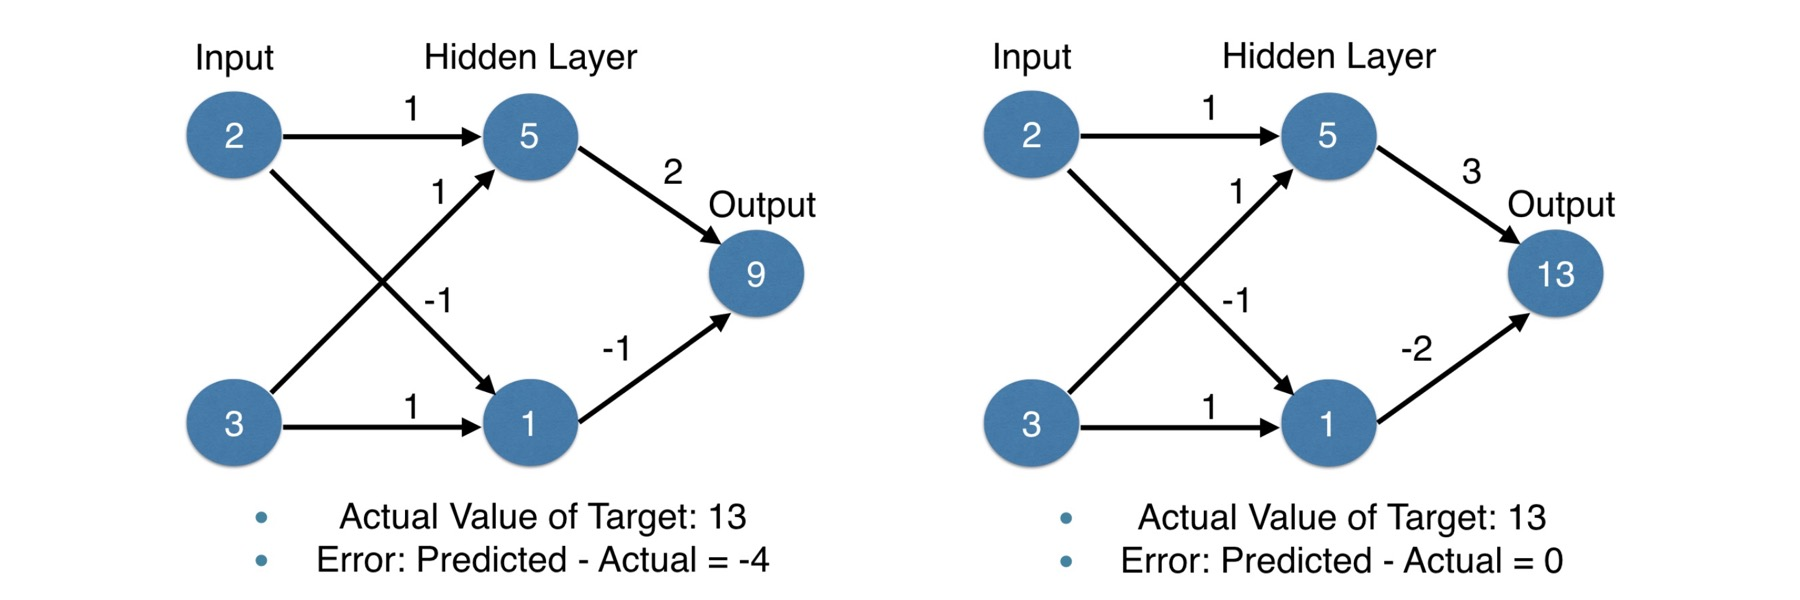
\includegraphics{../Figures/1. A baseline neural network.jpg}
\caption{A baseline neural network}
\end{figure}

    \hypertarget{note-2-predictions-with-multiple-points}{%
\subsection{\texorpdfstring{\texttt{{[}note-2{]}} Predictions with
multiple
points}{{[}note-2{]} Predictions with multiple points}}\label{note-2-predictions-with-multiple-points}}

\begin{itemize}
\item
  Making accurate predictions gets harder with more points.
\item
  At any set of weights, there are many values of the error
  corresponding to the many points that make predictions for.
\end{itemize}

    \hypertarget{note-3-loss-function}{%
\subsection{\texorpdfstring{\texttt{{[}note-3{]}} Loss
function}{{[}note-3{]} Loss function}}\label{note-3-loss-function}}

\begin{itemize}
\item
  Aggregates errors in predictions from many data points into a single
  number.
\item
  The loss function is a measure of the model's predictive performance.
\item
  A lower loss function value means a better model.
\item
  Goal: find the weights that give the lowest value for the loss
  function.
\item
  Gradient descent.
\end{itemize}

\begin{figure}
\centering
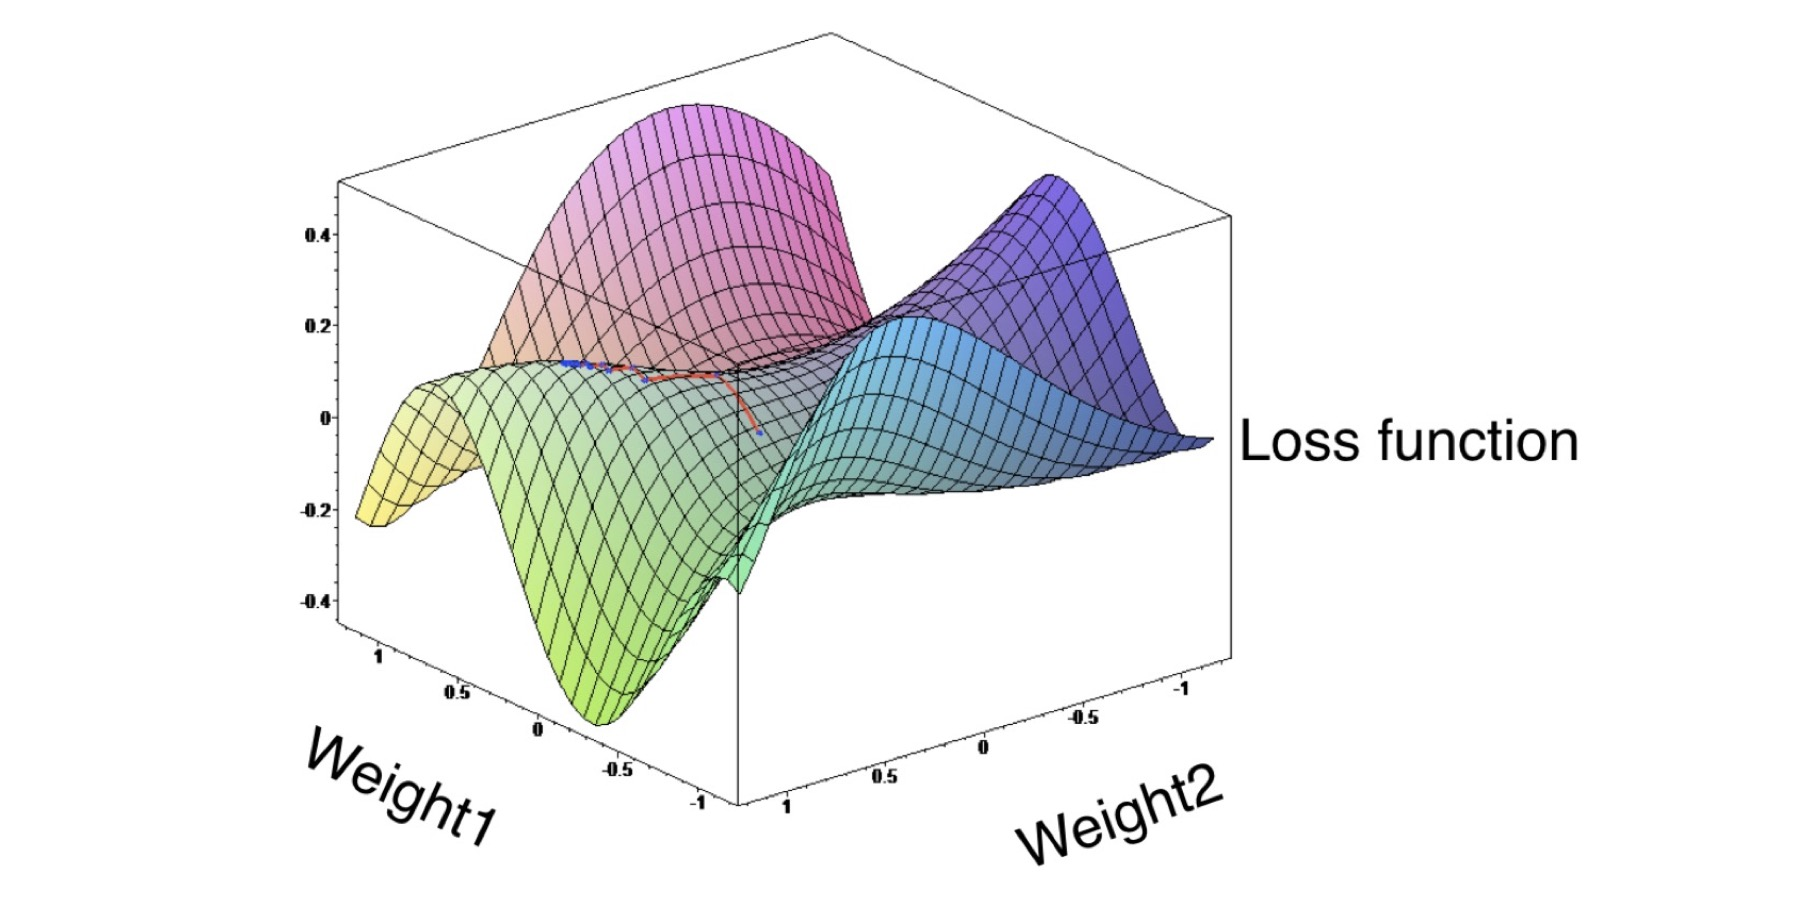
\includegraphics{../Figures/2. Loss function.jpg}
\caption{Loss function}
\end{figure}

    \hypertarget{note-4-gradient-descent}{%
\subsection{\texorpdfstring{\texttt{{[}note-4{]}} Gradient
descent}{{[}note-4{]} Gradient descent}}\label{note-4-gradient-descent}}

\begin{itemize}
\item
  Imagine starting in a pitch dark field.
\item
  Want to find the lowest point.
\item
  Feel the ground to see how it slopes.
\item
  Take a small step downhill.
\item
  Repeat until it is uphill in every direction.
\end{itemize}

    \hypertarget{note-5-gradient-descent-steps}{%
\subsection{\texorpdfstring{\texttt{{[}note-5{]}} Gradient descent
steps}{{[}note-5{]} Gradient descent steps}}\label{note-5-gradient-descent-steps}}

\begin{itemize}
\item
  Start at a random point.
\item
  Until arrived at somewhere flat:

  \begin{itemize}
  \item
    find the slope
  \item
    take a step downhill
  \end{itemize}
\end{itemize}

    \hypertarget{note-6-optimizing-a-model-with-a-single-weight}{%
\subsection{\texorpdfstring{\texttt{{[}note-6{]}} Optimizing a model
with a single
weight}{{[}note-6{]} Optimizing a model with a single weight}}\label{note-6-optimizing-a-model-with-a-single-weight}}

\begin{figure}
\centering
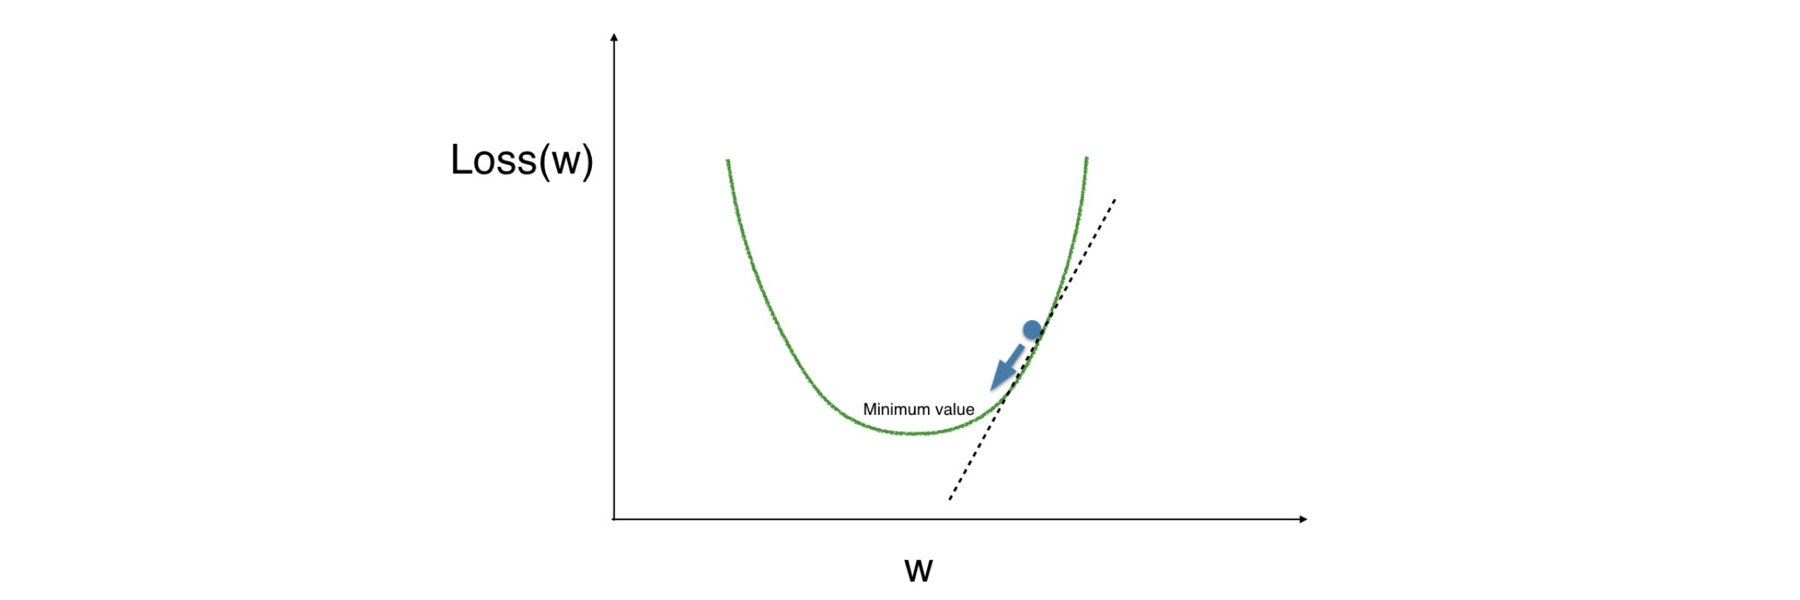
\includegraphics{../Figures/3. Optimizing a model with a single weight.jpg}
\caption{Optimizing a model with a single weight}
\end{figure}

    \hypertarget{quiz-1-calculating-model-errors}{%
\subsection{\texorpdfstring{\texttt{{[}quiz-1{]}} Calculating model
errors}{{[}quiz-1{]} Calculating model errors}}\label{quiz-1-calculating-model-errors}}

\begin{itemize}
\item
  Continue working with the network to predict transactions for a bank.
\item
  What is the error (\(error = predicted - actual\)) for the following
  network using the ReLU activation function when the input data is
  \([3, 2]\), and the actual value of the target, which tries to
  predict, is \(5\)? It may be helpful to get out a pen and piece of
  paper to calculate these values.

  \begin{figure}
  \centering
  
\includegraphics{../Figures/4. Calculating model errors.png}
  \caption{Calculating model errors}
  \end{figure}

  \(\Box\) \(5\).

  \(\Box\) \(6\).

  \(\boxtimes\) \(11\).

  \(\Box\) \(16\).
\end{itemize}

    \hypertarget{quiz-2-understanding-how-weights-change-model-accuracy}{%
\subsection{\texorpdfstring{\texttt{{[}quiz-2{]}} Understanding how
weights change model
accuracy}{{[}quiz-2{]} Understanding how weights change model accuracy}}\label{quiz-2-understanding-how-weights-change-model-accuracy}}

\begin{itemize}
\item
  Imagine making a prediction for a single data point. The actual value
  of the target is \(7\). The weight going from \texttt{node\_0} to the
  output is \(2\), as shown below. If it is increased slightly, changing
  it to \(2.01\), would the predictions become more accurate, less
  accurate, or stay the same?

  \begin{figure}
  \centering
  
\includegraphics{../Figures/5. Understanding how weights change model accuracy.png}
  \caption{Understanding how weights change model accuracy}
  \end{figure}

  \(\Box\) More accurate.

  \(\boxtimes\) Less accurate.

  \(\Box\) Stay the same.
\end{itemize}

    \hypertarget{task-1-coding-how-weight-changes-affect-the-accuracy}{%
\subsection{\texorpdfstring{\texttt{{[}task-1{]}} Coding how weight
changes affect the
accuracy}{{[}task-1{]} Coding how weight changes affect the accuracy}}\label{task-1-coding-how-weight-changes-affect-the-accuracy}}

\(\blacktriangleright\) \textbf{Task diagram}

\begin{figure}
\centering

\includegraphics{../Figures/6. Coding how weight changes affect the accuracy.png}
\caption{Coding how weight changes affect the accuracy}
\end{figure}

    \(\blacktriangleright\) \textbf{Package pre-loading}

    \begin{tcolorbox}[breakable, size=fbox, boxrule=1pt, pad at break*=1mm,colback=cellbackground, colframe=cellborder]
\prompt{In}{incolor}{1}{\boxspacing}
\begin{Verbatim}[commandchars=\\\{\}]
\PY{k+kn}{import} \PY{n+nn}{numpy} \PY{k}{as} \PY{n+nn}{np}
\end{Verbatim}
\end{tcolorbox}

    \(\blacktriangleright\) \textbf{Code pre-loading}

    \begin{tcolorbox}[breakable, size=fbox, boxrule=1pt, pad at break*=1mm,colback=cellbackground, colframe=cellborder]
\prompt{In}{incolor}{2}{\boxspacing}
\begin{Verbatim}[commandchars=\\\{\}]
\PY{k}{def} \PY{n+nf}{predict\PYZus{}with\PYZus{}network}\PY{p}{(}\PY{n}{input\PYZus{}data\PYZus{}point}\PY{p}{,} \PY{n}{weights}\PY{p}{)}\PY{p}{:}
    \PY{n}{node\PYZus{}0\PYZus{}input} \PY{o}{=} \PY{p}{(}\PY{n}{input\PYZus{}data\PYZus{}point} \PY{o}{*} \PY{n}{weights}\PY{p}{[}\PY{l+s+s1}{\PYZsq{}}\PY{l+s+s1}{node\PYZus{}0}\PY{l+s+s1}{\PYZsq{}}\PY{p}{]}\PY{p}{)}\PY{o}{.}\PY{n}{sum}\PY{p}{(}\PY{p}{)}
    \PY{n}{node\PYZus{}0\PYZus{}output} \PY{o}{=} \PY{n}{relu}\PY{p}{(}\PY{n}{node\PYZus{}0\PYZus{}input}\PY{p}{)}

    \PY{n}{node\PYZus{}1\PYZus{}input} \PY{o}{=} \PY{p}{(}\PY{n}{input\PYZus{}data\PYZus{}point} \PY{o}{*} \PY{n}{weights}\PY{p}{[}\PY{l+s+s1}{\PYZsq{}}\PY{l+s+s1}{node\PYZus{}1}\PY{l+s+s1}{\PYZsq{}}\PY{p}{]}\PY{p}{)}\PY{o}{.}\PY{n}{sum}\PY{p}{(}\PY{p}{)}
    \PY{n}{node\PYZus{}1\PYZus{}output} \PY{o}{=} \PY{n}{relu}\PY{p}{(}\PY{n}{node\PYZus{}1\PYZus{}input}\PY{p}{)}

    \PY{n}{hidden\PYZus{}layer\PYZus{}values} \PY{o}{=} \PY{n}{np}\PY{o}{.}\PY{n}{array}\PY{p}{(}\PY{p}{[}\PY{n}{node\PYZus{}0\PYZus{}output}\PY{p}{,} \PY{n}{node\PYZus{}1\PYZus{}output}\PY{p}{]}\PY{p}{)}
    \PY{n}{input\PYZus{}to\PYZus{}final\PYZus{}layer} \PY{o}{=} \PY{p}{(}\PY{n}{hidden\PYZus{}layer\PYZus{}values} \PY{o}{*} \PY{n}{weights}\PY{p}{[}\PY{l+s+s1}{\PYZsq{}}\PY{l+s+s1}{output}\PY{l+s+s1}{\PYZsq{}}\PY{p}{]}\PY{p}{)}\PY{o}{.}\PY{n}{sum}\PY{p}{(}\PY{p}{)}
    \PY{n}{model\PYZus{}output} \PY{o}{=} \PY{n}{relu}\PY{p}{(}\PY{n}{input\PYZus{}to\PYZus{}final\PYZus{}layer}\PY{p}{)}

    \PY{k}{return} \PY{p}{(}\PY{n}{model\PYZus{}output}\PY{p}{)}


\PY{k}{def} \PY{n+nf}{relu}\PY{p}{(}\PY{n}{my\PYZus{}input}\PY{p}{)}\PY{p}{:}
    \PY{k}{return} \PY{p}{(}\PY{n+nb}{max}\PY{p}{(}\PY{l+m+mi}{0}\PY{p}{,} \PY{n}{my\PYZus{}input}\PY{p}{)}\PY{p}{)}
\end{Verbatim}
\end{tcolorbox}

    \(\blacktriangleright\) \textbf{Task practice}

    \begin{tcolorbox}[breakable, size=fbox, boxrule=1pt, pad at break*=1mm,colback=cellbackground, colframe=cellborder]
\prompt{In}{incolor}{3}{\boxspacing}
\begin{Verbatim}[commandchars=\\\{\}]
\PY{c+c1}{\PYZsh{} The data point you will make a prediction for}
\PY{n}{input\PYZus{}data} \PY{o}{=} \PY{n}{np}\PY{o}{.}\PY{n}{array}\PY{p}{(}\PY{p}{[}\PY{l+m+mi}{0}\PY{p}{,} \PY{l+m+mi}{3}\PY{p}{]}\PY{p}{)}

\PY{c+c1}{\PYZsh{} Sample weights}
\PY{n}{weights\PYZus{}0} \PY{o}{=} \PY{p}{\PYZob{}}\PY{l+s+s1}{\PYZsq{}}\PY{l+s+s1}{node\PYZus{}0}\PY{l+s+s1}{\PYZsq{}}\PY{p}{:} \PY{p}{[}\PY{l+m+mi}{2}\PY{p}{,} \PY{l+m+mi}{1}\PY{p}{]}\PY{p}{,} \PY{l+s+s1}{\PYZsq{}}\PY{l+s+s1}{node\PYZus{}1}\PY{l+s+s1}{\PYZsq{}}\PY{p}{:} \PY{p}{[}\PY{l+m+mi}{1}\PY{p}{,} \PY{l+m+mi}{2}\PY{p}{]}\PY{p}{,} \PY{l+s+s1}{\PYZsq{}}\PY{l+s+s1}{output}\PY{l+s+s1}{\PYZsq{}}\PY{p}{:} \PY{p}{[}\PY{l+m+mi}{1}\PY{p}{,} \PY{l+m+mi}{1}\PY{p}{]}\PY{p}{\PYZcb{}}

\PY{c+c1}{\PYZsh{} The actual target value, used to calculate the error}
\PY{n}{target\PYZus{}actual} \PY{o}{=} \PY{l+m+mi}{3}

\PY{c+c1}{\PYZsh{} Make prediction using original weights}
\PY{n}{model\PYZus{}output\PYZus{}0} \PY{o}{=} \PY{n}{predict\PYZus{}with\PYZus{}network}\PY{p}{(}\PY{n}{input\PYZus{}data}\PY{p}{,} \PY{n}{weights\PYZus{}0}\PY{p}{)}

\PY{c+c1}{\PYZsh{} Calculate error: error\PYZus{}0}
\PY{n}{error\PYZus{}0} \PY{o}{=} \PY{n}{model\PYZus{}output\PYZus{}0} \PY{o}{\PYZhy{}} \PY{n}{target\PYZus{}actual}

\PY{c+c1}{\PYZsh{} Create weights that cause the network to make perfect prediction (3): weights\PYZus{}1}
\PY{n}{weights\PYZus{}1} \PY{o}{=} \PY{p}{\PYZob{}}\PY{l+s+s1}{\PYZsq{}}\PY{l+s+s1}{node\PYZus{}0}\PY{l+s+s1}{\PYZsq{}}\PY{p}{:} \PY{p}{[}\PY{l+m+mi}{2}\PY{p}{,} \PY{l+m+mi}{1}\PY{p}{]}\PY{p}{,} \PY{l+s+s1}{\PYZsq{}}\PY{l+s+s1}{node\PYZus{}1}\PY{l+s+s1}{\PYZsq{}}\PY{p}{:} \PY{p}{[}\PY{l+m+mi}{1}\PY{p}{,} \PY{l+m+mi}{0}\PY{p}{]}\PY{p}{,} \PY{l+s+s1}{\PYZsq{}}\PY{l+s+s1}{output}\PY{l+s+s1}{\PYZsq{}}\PY{p}{:} \PY{p}{[}\PY{l+m+mi}{1}\PY{p}{,} \PY{l+m+mi}{1}\PY{p}{]}\PY{p}{\PYZcb{}}

\PY{c+c1}{\PYZsh{} Make prediction using new weights: model\PYZus{}output\PYZus{}1}
\PY{n}{model\PYZus{}output\PYZus{}1} \PY{o}{=} \PY{n}{predict\PYZus{}with\PYZus{}network}\PY{p}{(}\PY{n}{input\PYZus{}data}\PY{p}{,} \PY{n}{weights\PYZus{}1}\PY{p}{)}

\PY{c+c1}{\PYZsh{} Calculate error: error\PYZus{}1}
\PY{n}{error\PYZus{}1} \PY{o}{=} \PY{n}{model\PYZus{}output\PYZus{}1} \PY{o}{\PYZhy{}} \PY{n}{target\PYZus{}actual}

\PY{c+c1}{\PYZsh{} Print error\PYZus{}0 and error\PYZus{}1}
\PY{n+nb}{print}\PY{p}{(}\PY{n}{error\PYZus{}0}\PY{p}{)}
\PY{n+nb}{print}\PY{p}{(}\PY{n}{error\PYZus{}1}\PY{p}{)}
\end{Verbatim}
\end{tcolorbox}

    \begin{Verbatim}[commandchars=\\\{\}]
6
0
    \end{Verbatim}

    \hypertarget{task-2-scaling-up-to-multiple-data-points}{%
\subsection{\texorpdfstring{\texttt{{[}task-2{]}} Scaling up to multiple
data
points}{{[}task-2{]} Scaling up to multiple data points}}\label{task-2-scaling-up-to-multiple-data-points}}

\(\blacktriangleright\) \textbf{Data pre-loading}

    \begin{tcolorbox}[breakable, size=fbox, boxrule=1pt, pad at break*=1mm,colback=cellbackground, colframe=cellborder]
\prompt{In}{incolor}{4}{\boxspacing}
\begin{Verbatim}[commandchars=\\\{\}]
\PY{n}{input\PYZus{}data} \PY{o}{=} \PY{p}{[}
    \PY{n}{np}\PY{o}{.}\PY{n}{array}\PY{p}{(}\PY{p}{[}\PY{l+m+mi}{0}\PY{p}{,} \PY{l+m+mi}{3}\PY{p}{]}\PY{p}{)}\PY{p}{,}
    \PY{n}{np}\PY{o}{.}\PY{n}{array}\PY{p}{(}\PY{p}{[}\PY{l+m+mi}{1}\PY{p}{,} \PY{l+m+mi}{2}\PY{p}{]}\PY{p}{)}\PY{p}{,}
    \PY{n}{np}\PY{o}{.}\PY{n}{array}\PY{p}{(}\PY{p}{[}\PY{o}{\PYZhy{}}\PY{l+m+mi}{1}\PY{p}{,} \PY{o}{\PYZhy{}}\PY{l+m+mi}{2}\PY{p}{]}\PY{p}{)}\PY{p}{,}
    \PY{n}{np}\PY{o}{.}\PY{n}{array}\PY{p}{(}\PY{p}{[}\PY{l+m+mi}{4}\PY{p}{,} \PY{l+m+mi}{0}\PY{p}{]}\PY{p}{)}
\PY{p}{]}

\PY{n}{weights\PYZus{}0} \PY{o}{=} \PY{p}{\PYZob{}}
    \PY{l+s+s1}{\PYZsq{}}\PY{l+s+s1}{node\PYZus{}0}\PY{l+s+s1}{\PYZsq{}}\PY{p}{:} \PY{n}{np}\PY{o}{.}\PY{n}{array}\PY{p}{(}\PY{p}{[}\PY{l+m+mi}{2}\PY{p}{,} \PY{l+m+mi}{1}\PY{p}{]}\PY{p}{)}\PY{p}{,}
    \PY{l+s+s1}{\PYZsq{}}\PY{l+s+s1}{node\PYZus{}1}\PY{l+s+s1}{\PYZsq{}}\PY{p}{:} \PY{n}{np}\PY{o}{.}\PY{n}{array}\PY{p}{(}\PY{p}{[}\PY{l+m+mi}{1}\PY{p}{,} \PY{l+m+mi}{2}\PY{p}{]}\PY{p}{)}\PY{p}{,}
    \PY{l+s+s1}{\PYZsq{}}\PY{l+s+s1}{output}\PY{l+s+s1}{\PYZsq{}}\PY{p}{:} \PY{n}{np}\PY{o}{.}\PY{n}{array}\PY{p}{(}\PY{p}{[}\PY{l+m+mi}{1}\PY{p}{,} \PY{l+m+mi}{1}\PY{p}{]}\PY{p}{)}
\PY{p}{\PYZcb{}}

\PY{n}{weights\PYZus{}1} \PY{o}{=} \PY{p}{\PYZob{}}
    \PY{l+s+s1}{\PYZsq{}}\PY{l+s+s1}{node\PYZus{}0}\PY{l+s+s1}{\PYZsq{}}\PY{p}{:} \PY{n}{np}\PY{o}{.}\PY{n}{array}\PY{p}{(}\PY{p}{[}\PY{l+m+mi}{2}\PY{p}{,} \PY{l+m+mi}{1}\PY{p}{]}\PY{p}{)}\PY{p}{,}
    \PY{l+s+s1}{\PYZsq{}}\PY{l+s+s1}{node\PYZus{}1}\PY{l+s+s1}{\PYZsq{}}\PY{p}{:} \PY{n}{np}\PY{o}{.}\PY{n}{array}\PY{p}{(}\PY{p}{[}\PY{l+m+mf}{1.}\PY{p}{,} \PY{l+m+mf}{1.5}\PY{p}{]}\PY{p}{)}\PY{p}{,}
    \PY{l+s+s1}{\PYZsq{}}\PY{l+s+s1}{output}\PY{l+s+s1}{\PYZsq{}}\PY{p}{:} \PY{n}{np}\PY{o}{.}\PY{n}{array}\PY{p}{(}\PY{p}{[}\PY{l+m+mf}{1.}\PY{p}{,} \PY{l+m+mf}{1.5}\PY{p}{]}\PY{p}{)}
\PY{p}{\PYZcb{}}

\PY{n}{target\PYZus{}actuals} \PY{o}{=} \PY{p}{[}\PY{l+m+mi}{1}\PY{p}{,} \PY{l+m+mi}{3}\PY{p}{,} \PY{l+m+mi}{5}\PY{p}{,} \PY{l+m+mi}{7}\PY{p}{]}
\end{Verbatim}
\end{tcolorbox}

    \(\blacktriangleright\) \textbf{Task practice}

    \begin{tcolorbox}[breakable, size=fbox, boxrule=1pt, pad at break*=1mm,colback=cellbackground, colframe=cellborder]
\prompt{In}{incolor}{5}{\boxspacing}
\begin{Verbatim}[commandchars=\\\{\}]
\PY{k+kn}{from} \PY{n+nn}{sklearn}\PY{n+nn}{.}\PY{n+nn}{metrics} \PY{k+kn}{import} \PY{n}{mean\PYZus{}squared\PYZus{}error}

\PY{c+c1}{\PYZsh{} Create model\PYZus{}output\PYZus{}0}
\PY{n}{model\PYZus{}output\PYZus{}0} \PY{o}{=} \PY{p}{[}\PY{p}{]}
\PY{c+c1}{\PYZsh{} Create model\PYZus{}output\PYZus{}1}
\PY{n}{model\PYZus{}output\PYZus{}1} \PY{o}{=} \PY{p}{[}\PY{p}{]}

\PY{c+c1}{\PYZsh{} Loop over input\PYZus{}data}
\PY{k}{for} \PY{n}{row} \PY{o+ow}{in} \PY{n}{input\PYZus{}data}\PY{p}{:}
    \PY{c+c1}{\PYZsh{} Append prediction to model\PYZus{}output\PYZus{}0}
    \PY{n}{model\PYZus{}output\PYZus{}0}\PY{o}{.}\PY{n}{append}\PY{p}{(}\PY{n}{predict\PYZus{}with\PYZus{}network}\PY{p}{(}\PY{n}{row}\PY{p}{,} \PY{n}{weights\PYZus{}0}\PY{p}{)}\PY{p}{)}

    \PY{c+c1}{\PYZsh{} Append prediction to model\PYZus{}output\PYZus{}1}
    \PY{n}{model\PYZus{}output\PYZus{}1}\PY{o}{.}\PY{n}{append}\PY{p}{(}\PY{n}{predict\PYZus{}with\PYZus{}network}\PY{p}{(}\PY{n}{row}\PY{p}{,} \PY{n}{weights\PYZus{}1}\PY{p}{)}\PY{p}{)}

\PY{c+c1}{\PYZsh{} Calculate the mean squared error for model\PYZus{}output\PYZus{}0: mse\PYZus{}0}
\PY{n}{mse\PYZus{}0} \PY{o}{=} \PY{n}{mean\PYZus{}squared\PYZus{}error}\PY{p}{(}\PY{n}{target\PYZus{}actuals}\PY{p}{,} \PY{n}{model\PYZus{}output\PYZus{}0}\PY{p}{)}

\PY{c+c1}{\PYZsh{} Calculate the mean squared error for model\PYZus{}output\PYZus{}1: mse\PYZus{}1}
\PY{n}{mse\PYZus{}1} \PY{o}{=} \PY{n}{mean\PYZus{}squared\PYZus{}error}\PY{p}{(}\PY{n}{target\PYZus{}actuals}\PY{p}{,} \PY{n}{model\PYZus{}output\PYZus{}1}\PY{p}{)}

\PY{c+c1}{\PYZsh{} Print mse\PYZus{}0 and mse\PYZus{}1}
\PY{n+nb}{print}\PY{p}{(}\PY{l+s+s2}{\PYZdq{}}\PY{l+s+s2}{Mean squared error with weights\PYZus{}0: }\PY{l+s+si}{\PYZpc{}f}\PY{l+s+s2}{\PYZdq{}} \PY{o}{\PYZpc{}} \PY{n}{mse\PYZus{}0}\PY{p}{)}
\PY{n+nb}{print}\PY{p}{(}\PY{l+s+s2}{\PYZdq{}}\PY{l+s+s2}{Mean squared error with weights\PYZus{}1: }\PY{l+s+si}{\PYZpc{}f}\PY{l+s+s2}{\PYZdq{}} \PY{o}{\PYZpc{}} \PY{n}{mse\PYZus{}1}\PY{p}{)}
\end{Verbatim}
\end{tcolorbox}

    \begin{Verbatim}[commandchars=\\\{\}]
Mean squared error with weights\_0: 37.500000
Mean squared error with weights\_1: 49.890625
    \end{Verbatim}

    \hypertarget{gradient-descent}{%
\section{Gradient descent}\label{gradient-descent}}

    \hypertarget{note-1-gradient-descent}{%
\subsection{\texorpdfstring{\texttt{{[}note-1{]}} Gradient
descent}{{[}note-1{]} Gradient descent}}\label{note-1-gradient-descent}}

\begin{itemize}
\item
  If the slope is positive:

  \begin{itemize}
  \item
    going opposite the slope means moving to lower numbers
  \item
    subtract the slope from the current value
  \item
    too big a step might lead astray
  \end{itemize}
\item
  Solution: \emph{learning rate}

  \begin{itemize}
  \tightlist
  \item
    update each weight by subtracting \(learning\ rate \times slope\)
  \end{itemize}
\end{itemize}

\begin{figure}
\centering
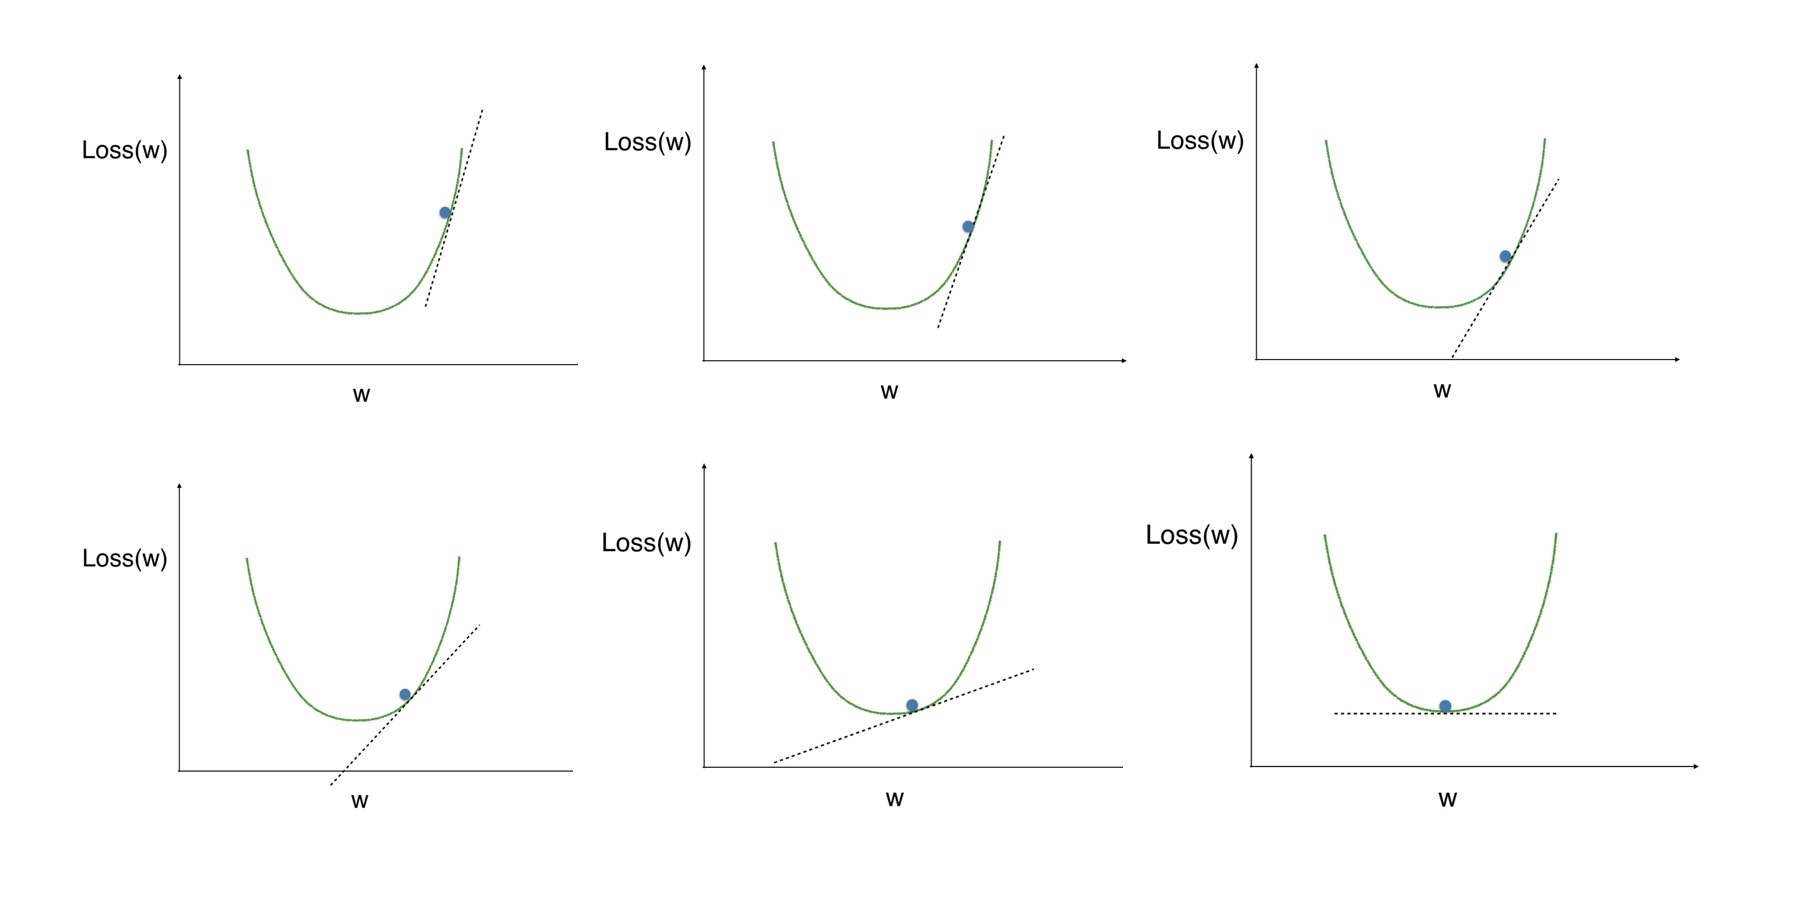
\includegraphics{../Figures/7. Gradient descent.jpg}
\caption{Gradient descent}
\end{figure}

    \hypertarget{note-2-slope-calculation-example}{%
\subsection{\texorpdfstring{\texttt{{[}note-2{]}} Slope calculation
example}{{[}note-2{]} Slope calculation example}}\label{note-2-slope-calculation-example}}

\begin{itemize}
\item
  To calculate the slope for a weight, need to multiply:

  \begin{itemize}
  \item
    the slope of the loss function with respect to value at the node
    which has been feed into
  \item
    the value of the node that feeds into the weight
  \item
    the slope of the activation function with respect to the value which
    has been feed into
  \end{itemize}
\item
  In this example, the slope of the mean-squared loss function with
  respect to prediction will be considered:
\end{itemize}

\begin{equation*}
    \begin{aligned}
        {MSE}^{\prime}\ &=\ \left({\left(Predicted\ Value\ -\ Actual\ Value\right)}^{2}\right)^{\prime}\\
        &=\ 2\ \cdot\ \left(Predicted\ Value\ -\ Actual\ Value\right)\\
        &=\ 2\ \cdot\ Error
    \end{aligned}
\end{equation*}

\begin{itemize}
\item
  In this example, the slope of the mean-squared loss function will be
  \(2 \cdot (6 - 10) = 2 \cdot (-4)\), the value of the node that feeds
  into the weight is \(3\), and no activation function needs to be
  considered. So the final multiplied slope for the weight will be
  \(2 \cdot (-4) \cdot 3 = -24\).
\item
  In this example, if the learning rate is \(0.01\), the new weight
  would be \(2 - 0.01 \cdot (-24) = 2.24\).
\end{itemize}

\begin{figure}
\centering

\includegraphics{../Figures/8. Slope calculation example.jpg}
\caption{Slope calculation example}
\end{figure}

    \hypertarget{note-3-network-with-two-inputs-affecting-prediction}{%
\subsection{\texorpdfstring{\texttt{{[}note-3{]}} Network with two
inputs affecting
prediction}{{[}note-3{]} Network with two inputs affecting prediction}}\label{note-3-network-with-two-inputs-affecting-prediction}}

\begin{figure}
\centering

\includegraphics{../Figures/9. Network with two inputs affecting prediction.jpg}
\caption{Network with two inputs affecting prediction}
\end{figure}

    \hypertarget{code-1-calculate-slopes-and-update-weights}{%
\subsection{\texorpdfstring{\texttt{{[}code-1{]}} Calculate slopes and
update
weights}{{[}code-1{]} Calculate slopes and update weights}}\label{code-1-calculate-slopes-and-update-weights}}

    \begin{tcolorbox}[breakable, size=fbox, boxrule=1pt, pad at break*=1mm,colback=cellbackground, colframe=cellborder]
\prompt{In}{incolor}{6}{\boxspacing}
\begin{Verbatim}[commandchars=\\\{\}]
\PY{k+kn}{import} \PY{n+nn}{numpy} \PY{k}{as} \PY{n+nn}{np}

\PY{n}{weights} \PY{o}{=} \PY{n}{np}\PY{o}{.}\PY{n}{array}\PY{p}{(}\PY{p}{[}\PY{l+m+mi}{1}\PY{p}{,} \PY{l+m+mi}{2}\PY{p}{]}\PY{p}{)}
\PY{n}{input\PYZus{}data} \PY{o}{=} \PY{n}{np}\PY{o}{.}\PY{n}{array}\PY{p}{(}\PY{p}{[}\PY{l+m+mi}{3}\PY{p}{,} \PY{l+m+mi}{4}\PY{p}{]}\PY{p}{)}
\PY{n}{target} \PY{o}{=} \PY{l+m+mi}{6}
\PY{n}{learning\PYZus{}rate} \PY{o}{=} \PY{l+m+mf}{0.01}

\PY{n}{preds} \PY{o}{=} \PY{p}{(}\PY{n}{weights} \PY{o}{*} \PY{n}{input\PYZus{}data}\PY{p}{)}\PY{o}{.}\PY{n}{sum}\PY{p}{(}\PY{p}{)}
\PY{n}{error} \PY{o}{=} \PY{n}{preds} \PY{o}{\PYZhy{}} \PY{n}{target}
\PY{n+nb}{print}\PY{p}{(}\PY{n}{error}\PY{p}{)}
\end{Verbatim}
\end{tcolorbox}

    \begin{Verbatim}[commandchars=\\\{\}]
5
    \end{Verbatim}

    \begin{tcolorbox}[breakable, size=fbox, boxrule=1pt, pad at break*=1mm,colback=cellbackground, colframe=cellborder]
\prompt{In}{incolor}{7}{\boxspacing}
\begin{Verbatim}[commandchars=\\\{\}]
\PY{n}{gradient} \PY{o}{=} \PY{l+m+mi}{2} \PY{o}{*} \PY{n}{input\PYZus{}data} \PY{o}{*} \PY{n}{error}
\PY{n}{gradient}
\end{Verbatim}
\end{tcolorbox}

            \begin{tcolorbox}[breakable, size=fbox, boxrule=.5pt, pad at break*=1mm, opacityfill=0]
\prompt{Out}{outcolor}{7}{\boxspacing}
\begin{Verbatim}[commandchars=\\\{\}]
array([30, 40])
\end{Verbatim}
\end{tcolorbox}
        
    \begin{tcolorbox}[breakable, size=fbox, boxrule=1pt, pad at break*=1mm,colback=cellbackground, colframe=cellborder]
\prompt{In}{incolor}{8}{\boxspacing}
\begin{Verbatim}[commandchars=\\\{\}]
\PY{n}{weights\PYZus{}updated} \PY{o}{=} \PY{n}{weights} \PY{o}{\PYZhy{}} \PY{n}{learning\PYZus{}rate} \PY{o}{*} \PY{n}{gradient}
\PY{n}{preds\PYZus{}updated} \PY{o}{=} \PY{p}{(}\PY{n}{weights\PYZus{}updated} \PY{o}{*} \PY{n}{input\PYZus{}data}\PY{p}{)}\PY{o}{.}\PY{n}{sum}\PY{p}{(}\PY{p}{)}
\PY{n}{error\PYZus{}updated} \PY{o}{=} \PY{n}{preds\PYZus{}updated} \PY{o}{\PYZhy{}} \PY{n}{target}
\PY{n+nb}{print}\PY{p}{(}\PY{n}{error\PYZus{}updated}\PY{p}{)}
\end{Verbatim}
\end{tcolorbox}

    \begin{Verbatim}[commandchars=\\\{\}]
2.5
    \end{Verbatim}

    \hypertarget{task-1-calculating-slopes}{%
\subsection{\texorpdfstring{\texttt{{[}task-1{]}} Calculating
slopes}{{[}task-1{]} Calculating slopes}}\label{task-1-calculating-slopes}}

\(\blacktriangleright\) \textbf{Package pre-loading}

    \begin{tcolorbox}[breakable, size=fbox, boxrule=1pt, pad at break*=1mm,colback=cellbackground, colframe=cellborder]
\prompt{In}{incolor}{9}{\boxspacing}
\begin{Verbatim}[commandchars=\\\{\}]
\PY{k+kn}{import} \PY{n+nn}{numpy} \PY{k}{as} \PY{n+nn}{np}
\end{Verbatim}
\end{tcolorbox}

    \(\blacktriangleright\) \textbf{Data pre-loading}

    \begin{tcolorbox}[breakable, size=fbox, boxrule=1pt, pad at break*=1mm,colback=cellbackground, colframe=cellborder]
\prompt{In}{incolor}{10}{\boxspacing}
\begin{Verbatim}[commandchars=\\\{\}]
\PY{n}{input\PYZus{}data} \PY{o}{=} \PY{n}{np}\PY{o}{.}\PY{n}{array}\PY{p}{(}\PY{p}{[}\PY{l+m+mi}{1}\PY{p}{,} \PY{l+m+mi}{2}\PY{p}{,} \PY{l+m+mi}{3}\PY{p}{]}\PY{p}{)}

\PY{n}{weights} \PY{o}{=} \PY{n}{np}\PY{o}{.}\PY{n}{array}\PY{p}{(}\PY{p}{[}\PY{l+m+mi}{0}\PY{p}{,} \PY{l+m+mi}{2}\PY{p}{,} \PY{l+m+mi}{1}\PY{p}{]}\PY{p}{)}

\PY{n}{target} \PY{o}{=} \PY{l+m+mi}{0}
\end{Verbatim}
\end{tcolorbox}

    \(\blacktriangleright\) \textbf{Task practice}

    \begin{tcolorbox}[breakable, size=fbox, boxrule=1pt, pad at break*=1mm,colback=cellbackground, colframe=cellborder]
\prompt{In}{incolor}{11}{\boxspacing}
\begin{Verbatim}[commandchars=\\\{\}]
\PY{c+c1}{\PYZsh{} Calculate the predictions: preds}
\PY{n}{preds} \PY{o}{=} \PY{p}{(}\PY{n}{weights} \PY{o}{*} \PY{n}{input\PYZus{}data}\PY{p}{)}\PY{o}{.}\PY{n}{sum}\PY{p}{(}\PY{p}{)}

\PY{c+c1}{\PYZsh{} Calculate the error: error}
\PY{n}{error} \PY{o}{=} \PY{n}{preds} \PY{o}{\PYZhy{}} \PY{n}{target}

\PY{c+c1}{\PYZsh{} Calculate the slope: slope}
\PY{n}{slope} \PY{o}{=} \PY{l+m+mi}{2} \PY{o}{*} \PY{n}{error} \PY{o}{*} \PY{n}{input\PYZus{}data}

\PY{c+c1}{\PYZsh{} Print the slope}
\PY{n+nb}{print}\PY{p}{(}\PY{n}{slope}\PY{p}{)}
\end{Verbatim}
\end{tcolorbox}

    \begin{Verbatim}[commandchars=\\\{\}]
[14 28 42]
    \end{Verbatim}

    \hypertarget{task-2-improving-model-weights}{%
\subsection{\texorpdfstring{\texttt{{[}task-2{]}} Improving model
weights}{{[}task-2{]} Improving model weights}}\label{task-2-improving-model-weights}}

\(\blacktriangleright\) \textbf{Task practice}

    \begin{tcolorbox}[breakable, size=fbox, boxrule=1pt, pad at break*=1mm,colback=cellbackground, colframe=cellborder]
\prompt{In}{incolor}{12}{\boxspacing}
\begin{Verbatim}[commandchars=\\\{\}]
\PY{c+c1}{\PYZsh{} Set the learning rate: learning\PYZus{}rate}
\PY{n}{learning\PYZus{}rate} \PY{o}{=} \PY{l+m+mf}{0.01}

\PY{c+c1}{\PYZsh{} Calculate the predictions: preds}
\PY{n}{preds} \PY{o}{=} \PY{p}{(}\PY{n}{weights} \PY{o}{*} \PY{n}{input\PYZus{}data}\PY{p}{)}\PY{o}{.}\PY{n}{sum}\PY{p}{(}\PY{p}{)}

\PY{c+c1}{\PYZsh{} Calculate the error: error}
\PY{n}{error} \PY{o}{=} \PY{n}{preds} \PY{o}{\PYZhy{}} \PY{n}{target}

\PY{c+c1}{\PYZsh{} Calculate the slope: slope}
\PY{n}{slope} \PY{o}{=} \PY{l+m+mi}{2} \PY{o}{*} \PY{n}{input\PYZus{}data} \PY{o}{*} \PY{n}{error}

\PY{c+c1}{\PYZsh{} Update the weights: weights\PYZus{}updated}
\PY{n}{weights\PYZus{}updated} \PY{o}{=} \PY{n}{weights} \PY{o}{\PYZhy{}} \PY{n}{learning\PYZus{}rate} \PY{o}{*} \PY{n}{slope}

\PY{c+c1}{\PYZsh{} Get updated predictions: preds\PYZus{}updated}
\PY{n}{preds\PYZus{}updated} \PY{o}{=} \PY{p}{(}\PY{n}{weights\PYZus{}updated} \PY{o}{*} \PY{n}{input\PYZus{}data}\PY{p}{)}\PY{o}{.}\PY{n}{sum}\PY{p}{(}\PY{p}{)}

\PY{c+c1}{\PYZsh{} Calculate updated error: error\PYZus{}updated}
\PY{n}{error\PYZus{}updated} \PY{o}{=} \PY{n}{preds\PYZus{}updated} \PY{o}{\PYZhy{}} \PY{n}{target}

\PY{c+c1}{\PYZsh{} Print the original error}
\PY{n+nb}{print}\PY{p}{(}\PY{n}{error}\PY{p}{)}

\PY{c+c1}{\PYZsh{} Print the updated error}
\PY{n+nb}{print}\PY{p}{(}\PY{n}{error\PYZus{}updated}\PY{p}{)}
\end{Verbatim}
\end{tcolorbox}

    \begin{Verbatim}[commandchars=\\\{\}]
7
5.04
    \end{Verbatim}

    \hypertarget{task-3-making-multiple-updates-to-weights}{%
\subsection{\texorpdfstring{\texttt{{[}task-3{]}} Making multiple
updates to
weights}{{[}task-3{]} Making multiple updates to weights}}\label{task-3-making-multiple-updates-to-weights}}

\(\blacktriangleright\) \textbf{Package pre-loading}

    \begin{tcolorbox}[breakable, size=fbox, boxrule=1pt, pad at break*=1mm,colback=cellbackground, colframe=cellborder]
\prompt{In}{incolor}{13}{\boxspacing}
\begin{Verbatim}[commandchars=\\\{\}]
\PY{k+kn}{import} \PY{n+nn}{matplotlib}\PY{n+nn}{.}\PY{n+nn}{pyplot} \PY{k}{as} \PY{n+nn}{plt}
\end{Verbatim}
\end{tcolorbox}

    \(\blacktriangleright\) \textbf{Code pre-loading}

    \begin{tcolorbox}[breakable, size=fbox, boxrule=1pt, pad at break*=1mm,colback=cellbackground, colframe=cellborder]
\prompt{In}{incolor}{14}{\boxspacing}
\begin{Verbatim}[commandchars=\\\{\}]
\PY{k}{def} \PY{n+nf}{get\PYZus{}error}\PY{p}{(}\PY{n}{input\PYZus{}data}\PY{p}{,} \PY{n}{target}\PY{p}{,} \PY{n}{weights}\PY{p}{)}\PY{p}{:}
    \PY{n}{preds} \PY{o}{=} \PY{p}{(}\PY{n}{weights} \PY{o}{*} \PY{n}{input\PYZus{}data}\PY{p}{)}\PY{o}{.}\PY{n}{sum}\PY{p}{(}\PY{p}{)}
    \PY{n}{error} \PY{o}{=} \PY{n}{preds} \PY{o}{\PYZhy{}} \PY{n}{target}
    \PY{k}{return} \PY{p}{(}\PY{n}{error}\PY{p}{)}


\PY{k}{def} \PY{n+nf}{get\PYZus{}slope}\PY{p}{(}\PY{n}{input\PYZus{}data}\PY{p}{,} \PY{n}{target}\PY{p}{,} \PY{n}{weights}\PY{p}{)}\PY{p}{:}
    \PY{n}{error} \PY{o}{=} \PY{n}{get\PYZus{}error}\PY{p}{(}\PY{n}{input\PYZus{}data}\PY{p}{,} \PY{n}{target}\PY{p}{,} \PY{n}{weights}\PY{p}{)}
    \PY{n}{slope} \PY{o}{=} \PY{l+m+mi}{2} \PY{o}{*} \PY{n}{input\PYZus{}data} \PY{o}{*} \PY{n}{error}
    \PY{k}{return} \PY{p}{(}\PY{n}{slope}\PY{p}{)}


\PY{k}{def} \PY{n+nf}{get\PYZus{}mse}\PY{p}{(}\PY{n}{input\PYZus{}data}\PY{p}{,} \PY{n}{target}\PY{p}{,} \PY{n}{weights}\PY{p}{)}\PY{p}{:}
    \PY{n}{errors} \PY{o}{=} \PY{n}{get\PYZus{}error}\PY{p}{(}\PY{n}{input\PYZus{}data}\PY{p}{,} \PY{n}{target}\PY{p}{,} \PY{n}{weights}\PY{p}{)}
    \PY{n}{mse} \PY{o}{=} \PY{n}{np}\PY{o}{.}\PY{n}{mean}\PY{p}{(}\PY{n}{errors}\PY{o}{*}\PY{o}{*}\PY{l+m+mi}{2}\PY{p}{)}
    \PY{k}{return} \PY{p}{(}\PY{n}{mse}\PY{p}{)}
\end{Verbatim}
\end{tcolorbox}

    \(\blacktriangleright\) \textbf{Task practice}

    \begin{tcolorbox}[breakable, size=fbox, boxrule=1pt, pad at break*=1mm,colback=cellbackground, colframe=cellborder]
\prompt{In}{incolor}{15}{\boxspacing}
\begin{Verbatim}[commandchars=\\\{\}]
\PY{n}{n\PYZus{}updates} \PY{o}{=} \PY{l+m+mi}{20}
\PY{n}{mse\PYZus{}hist} \PY{o}{=} \PY{p}{[}\PY{p}{]}

\PY{c+c1}{\PYZsh{} Iterate over the number of updates}
\PY{k}{for} \PY{n}{i} \PY{o+ow}{in} \PY{n+nb}{range}\PY{p}{(}\PY{n}{n\PYZus{}updates}\PY{p}{)}\PY{p}{:}
    \PY{c+c1}{\PYZsh{} Calculate the slope: slope}
    \PY{n}{slope} \PY{o}{=} \PY{n}{get\PYZus{}slope}\PY{p}{(}\PY{n}{input\PYZus{}data}\PY{p}{,} \PY{n}{target}\PY{p}{,} \PY{n}{weights}\PY{p}{)}

    \PY{c+c1}{\PYZsh{} Update the weights: weights}
    \PY{n}{weights} \PY{o}{=} \PY{n}{weights} \PY{o}{\PYZhy{}} \PY{l+m+mf}{0.01} \PY{o}{*} \PY{n}{slope}

    \PY{c+c1}{\PYZsh{} Calculate mse with new weights: mse}
    \PY{n}{mse} \PY{o}{=} \PY{n}{get\PYZus{}mse}\PY{p}{(}\PY{n}{input\PYZus{}data}\PY{p}{,} \PY{n}{target}\PY{p}{,} \PY{n}{weights}\PY{p}{)}

    \PY{c+c1}{\PYZsh{} Append the mse to mse\PYZus{}hist}
    \PY{n}{mse\PYZus{}hist}\PY{o}{.}\PY{n}{append}\PY{p}{(}\PY{n}{mse}\PY{p}{)}

\PY{c+c1}{\PYZsh{} Plot the mse history}
\PY{n}{plt}\PY{o}{.}\PY{n}{plot}\PY{p}{(}\PY{n}{mse\PYZus{}hist}\PY{p}{)}
\PY{n}{plt}\PY{o}{.}\PY{n}{xlabel}\PY{p}{(}\PY{l+s+s1}{\PYZsq{}}\PY{l+s+s1}{Iterations}\PY{l+s+s1}{\PYZsq{}}\PY{p}{)}
\PY{n}{plt}\PY{o}{.}\PY{n}{ylabel}\PY{p}{(}\PY{l+s+s1}{\PYZsq{}}\PY{l+s+s1}{Mean Squared Error}\PY{l+s+s1}{\PYZsq{}}\PY{p}{)}
\PY{n}{plt}\PY{o}{.}\PY{n}{show}\PY{p}{(}\PY{p}{)}
\end{Verbatim}
\end{tcolorbox}

    \begin{center}
    \adjustimage{max size={0.9\linewidth}{0.9\paperheight}}{output_42_0.png}
    \end{center}
    { \hspace*{\fill} \\}
    
    \hypertarget{backpropagation}{%
\section{Backpropagation}\label{backpropagation}}

    \hypertarget{note-1-backpropagation}{%
\subsection{\texorpdfstring{\texttt{{[}note-1{]}}
Backpropagation}{{[}note-1{]} Backpropagation}}\label{note-1-backpropagation}}

\begin{itemize}
\item
  Allows gradient descent to update all weights in the neural network
  (by getting gradients for all weights).
\item
  This algorithm comes from the chain rule of calculus.
\item
  Important to understand the process, but generally, there is a library
  available that implements this.
\end{itemize}

\begin{figure}
\centering

\includegraphics{../Figures/10. Backpropagation.jpg}
\caption{Backpropagation}
\end{figure}

    \hypertarget{note-2-backpropagation-process}{%
\subsection{\texorpdfstring{\texttt{{[}note-2{]}} Backpropagation
process}{{[}note-2{]} Backpropagation process}}\label{note-2-backpropagation-process}}

\begin{itemize}
\item
  Try to estimate the slope of the loss function with respect to each
  weight.
\item
  Do forward propagation to calculate predictions and errors.
\item
  Go back one layer at a time.
\item
  Gradients for weight is the product of:

  \begin{itemize}
  \item
    node value feeding into that weight
  \item
    the slope of the loss function with respect to node it feeds into
  \item
    the slope of activation function at the node it feeds into
  \end{itemize}
\item
  It is also necessary to keep track of the slopes of the loss function
  with respect to node values.
\item
  The slope of node values is the sum of the slopes for all weights that
  come out of them.
\end{itemize}

\begin{figure}
\centering
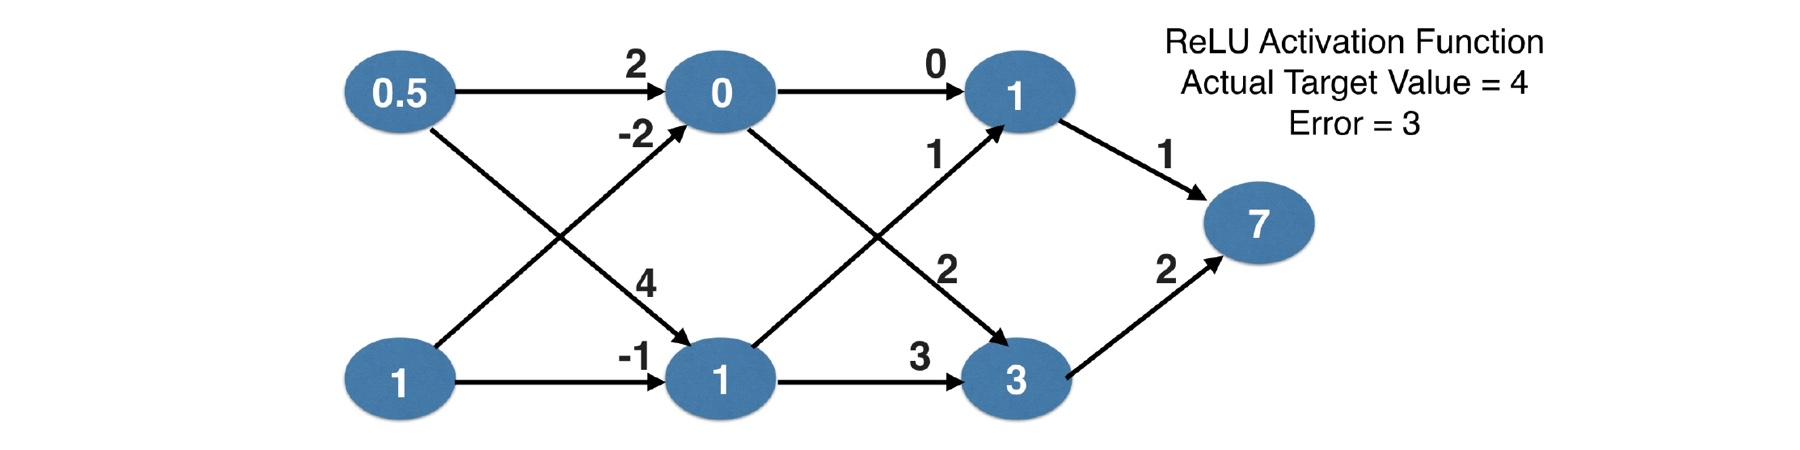
\includegraphics{../Figures/11. Backpropagation process.jpg}
\caption{Backpropagation process}
\end{figure}

    \hypertarget{quiz-1-the-relationship-between-the-forward-and-the-backward-propagation}{%
\subsection{\texorpdfstring{\texttt{{[}quiz-1{]}} The relationship
between the forward and the backward
propagation}{{[}quiz-1{]} The relationship between the forward and the backward propagation}}\label{quiz-1-the-relationship-between-the-forward-and-the-backward-propagation}}

\begin{itemize}
\item
  If it has been gone through \(4\) iterations of calculating slopes
  (using backward propagation) and then updated weights, how many times
  must the forward propagation have been done?

  \(\Box\) \(0\).

  \(\Box\) \(1\).

  \(\boxtimes\) \(4\).

  \(\Box\) \(8\).
\end{itemize}

    \hypertarget{quiz-2-thinking-about-backward-propagation}{%
\subsection{\texorpdfstring{\texttt{{[}quiz-2{]}} Thinking about
backward
propagation}{{[}quiz-2{]} Thinking about backward propagation}}\label{quiz-2-thinking-about-backward-propagation}}

\begin{itemize}
\item
  If the predictions were all exactly right, and the errors were all
  exactly \(0\), the slope of the loss function with respect to these
  predictions would also be \(0\). In that circumstance, which of the
  following statements would be correct?

  \(\boxtimes\) The updates to all weights in the network would also be
  \(0\).

  \(\Box\) The updates to all weights in the network would be dependent
  on the activation functions.

  \(\Box\) The updates to all weights in the network would be
  proportional to values from the input data.
\end{itemize}

    \hypertarget{backpropagation-in-practice}{%
\section{Backpropagation in
practice}\label{backpropagation-in-practice}}

    \hypertarget{note-1-calculating-slopes-associated-with-any-weight}{%
\subsection{\texorpdfstring{\texttt{{[}note-1{]}} Calculating slopes
associated with any
weight}{{[}note-1{]} Calculating slopes associated with any weight}}\label{note-1-calculating-slopes-associated-with-any-weight}}

\begin{itemize}
\item
  Gradients for weight is the product of:

  \begin{itemize}
  \item
    node value feeding into that weight
  \item
    the slope of activation function for the node being fed into
  \item
    the slope of the loss function with respect to the output node
  \end{itemize}
\end{itemize}

\begin{figure}
\centering
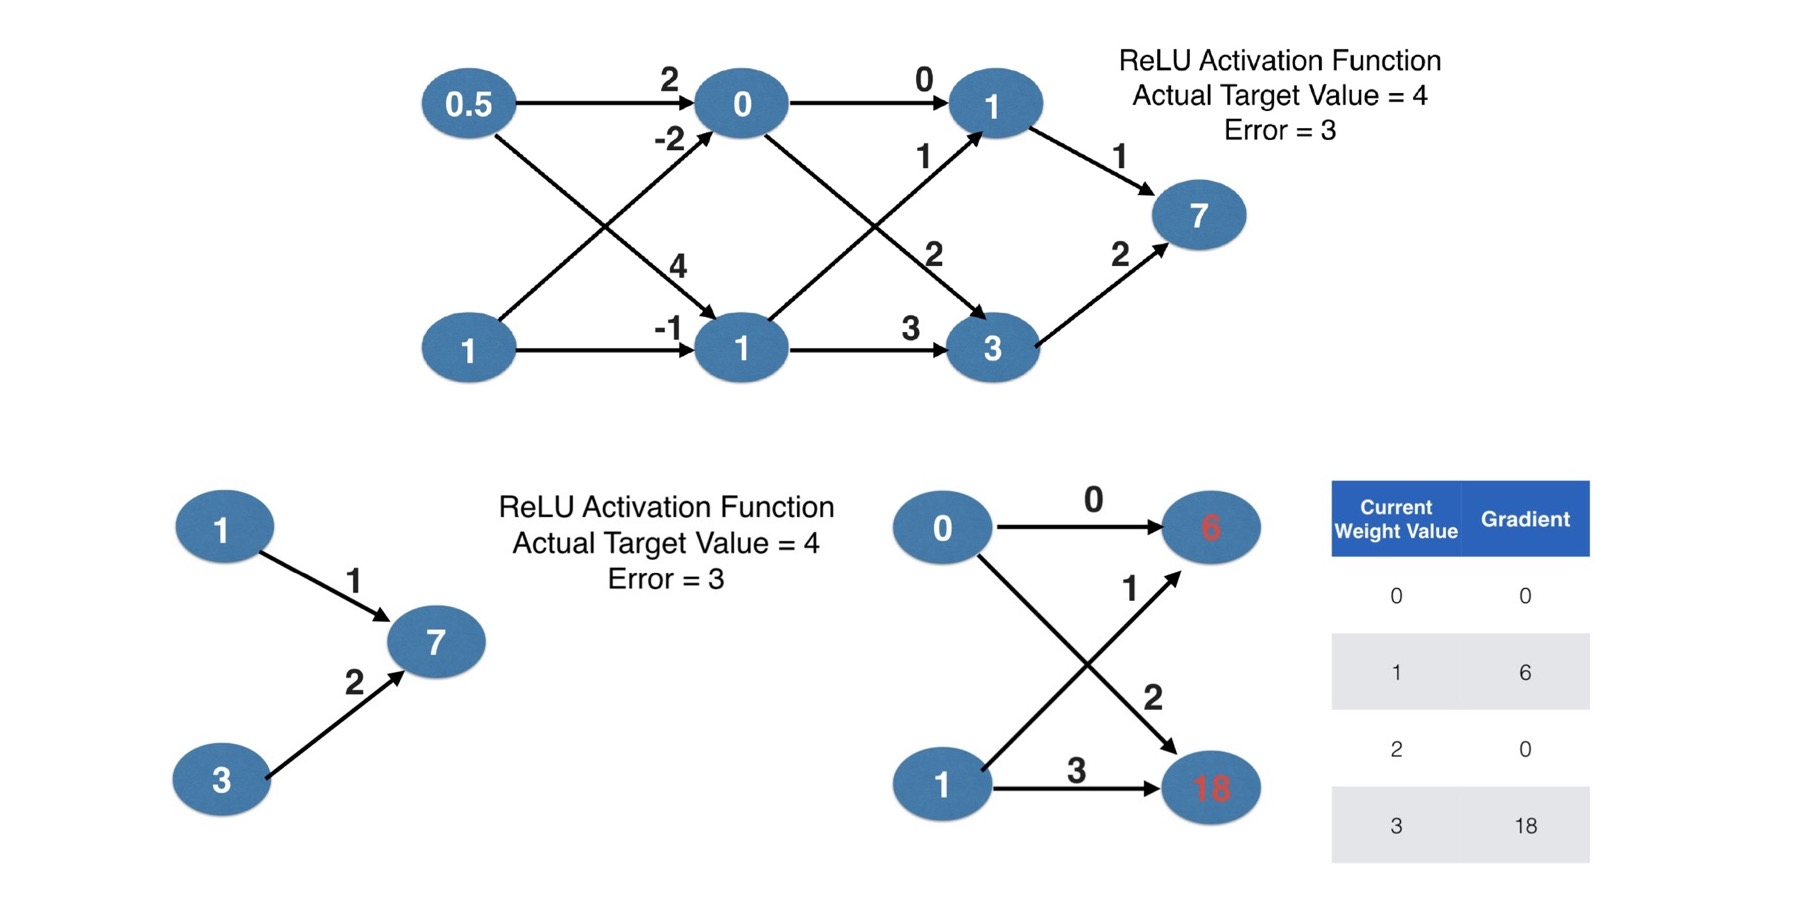
\includegraphics{../Figures/12. Calculating slopes associated with any weight.jpg}
\caption{Calculating slopes associated with any weight}
\end{figure}

    \hypertarget{note-2-recapitulation-of-backpropagation}{%
\subsection{\texorpdfstring{\texttt{{[}note-2{]}} Recapitulation of
backpropagation}{{[}note-2{]} Recapitulation of backpropagation}}\label{note-2-recapitulation-of-backpropagation}}

\begin{itemize}
\item
  Start at some random set of weights.
\item
  Use forward propagation to make a prediction.
\item
  Use backward propagation to calculate the slope of the loss function
  with respect to each weight.
\item
  Multiply that slope by the learning rate, and subtract from the
  current weights.
\item
  Keep going with that cycle until got to a flat part.
\end{itemize}

    \hypertarget{note-3-stochastic-gradient-descent}{%
\subsection{\texorpdfstring{\texttt{{[}note-3{]}} Stochastic gradient
descent}{{[}note-3{]} Stochastic gradient descent}}\label{note-3-stochastic-gradient-descent}}

\begin{itemize}
\item
  It is common to calculate slopes on only a subset of the data (a
  batch).
\item
  Use a different batch of data to calculate the next update.
\item
  Start over from the beginning once all data is used.
\item
  Each time through the training data is called an epoch.
\item
  When slopes are calculated on one batch at a time:

  \begin{itemize}
  \tightlist
  \item
    stochastic gradient descent
  \end{itemize}
\end{itemize}

    \hypertarget{quiz-1-a-round-of-backpropagation}{%
\subsection{\texorpdfstring{\texttt{{[}quiz-1{]}} A round of
backpropagation}{{[}quiz-1{]} A round of backpropagation}}\label{quiz-1-a-round-of-backpropagation}}

\begin{itemize}
\item
  In the network shown below, the forward propagation has been done, and
  node values calculated as part of the forward propagation are shown in
  white. The weights are shown in black. Layers after the question mark
  show the slopes calculated as part of the back-prop rather than the
  forward-prop values. Those slope values are shown in purple.
\item
  This network again uses the ReLU activation function, so the slope of
  the activation function is \(1\) for any node receiving a positive
  value as input. Assume the node being examined had a positive value
  (so the activation function's slope is \(1\)).

  \begin{figure}
  \centering
  
\includegraphics{../Figures/13. A round of backpropagation_1.png}
  \caption{A round of backpropagation\_1}
  \end{figure}
\item
  What is the slope needed to update the weight with the question mark?

  \begin{figure}
  \centering
  
\includegraphics{../Figures/14. A round of backpropagation_2.png}
  \caption{A round of backpropagation\_2}
  \end{figure}

  \(\Box\) \(0\).

  \(\Box\) \(2\).

  \(\boxtimes\) \(6\).

  \(\Box\) Not enough information.
\end{itemize}

    \hypertarget{requirements}{%
\section{Requirements}\label{requirements}}

    \begin{tcolorbox}[breakable, size=fbox, boxrule=1pt, pad at break*=1mm,colback=cellbackground, colframe=cellborder]
\prompt{In}{incolor}{16}{\boxspacing}
\begin{Verbatim}[commandchars=\\\{\}]
\PY{k+kn}{from} \PY{n+nn}{platform} \PY{k+kn}{import} \PY{n}{python\PYZus{}version}
\PY{k+kn}{import} \PY{n+nn}{sklearn}
\PY{k+kn}{import} \PY{n+nn}{matplotlib}

\PY{n}{python\PYZus{}version} \PY{o}{=} \PY{p}{(}\PY{l+s+s1}{\PYZsq{}}\PY{l+s+s1}{python==}\PY{l+s+si}{\PYZob{}\PYZcb{}}\PY{l+s+s1}{\PYZsq{}}\PY{o}{.}\PY{n}{format}\PY{p}{(}\PY{n}{python\PYZus{}version}\PY{p}{(}\PY{p}{)}\PY{p}{)}\PY{p}{)}
\PY{n}{numpy\PYZus{}version} \PY{o}{=} \PY{p}{(}\PY{l+s+s1}{\PYZsq{}}\PY{l+s+s1}{numpy==}\PY{l+s+si}{\PYZob{}\PYZcb{}}\PY{l+s+s1}{\PYZsq{}}\PY{o}{.}\PY{n}{format}\PY{p}{(}\PY{n}{np}\PY{o}{.}\PY{n}{\PYZus{}\PYZus{}version\PYZus{}\PYZus{}}\PY{p}{)}\PY{p}{)}
\PY{n}{scikit\PYZus{}learn\PYZus{}version} \PY{o}{=} \PY{p}{(}\PY{l+s+s1}{\PYZsq{}}\PY{l+s+s1}{scikit\PYZhy{}learn==}\PY{l+s+si}{\PYZob{}\PYZcb{}}\PY{l+s+s1}{\PYZsq{}}\PY{o}{.}\PY{n}{format}\PY{p}{(}\PY{n}{sklearn}\PY{o}{.}\PY{n}{\PYZus{}\PYZus{}version\PYZus{}\PYZus{}}\PY{p}{)}\PY{p}{)}
\PY{n}{matplotlib\PYZus{}version} \PY{o}{=} \PY{p}{(}\PY{l+s+s1}{\PYZsq{}}\PY{l+s+s1}{matplotlib==}\PY{l+s+si}{\PYZob{}\PYZcb{}}\PY{l+s+s1}{\PYZsq{}}\PY{o}{.}\PY{n}{format}\PY{p}{(}\PY{n}{matplotlib}\PY{o}{.}\PY{n}{\PYZus{}\PYZus{}version\PYZus{}\PYZus{}}\PY{p}{)}\PY{p}{)}

\PY{n}{writepath} \PY{o}{=} \PY{l+s+s1}{\PYZsq{}}\PY{l+s+s1}{../../requirements.txt}\PY{l+s+s1}{\PYZsq{}}
\PY{n}{requirements} \PY{o}{=} \PY{p}{[}\PY{p}{]}
\PY{n}{packages} \PY{o}{=} \PY{p}{[}\PY{n}{numpy\PYZus{}version}\PY{p}{,} \PY{n}{scikit\PYZus{}learn\PYZus{}version}\PY{p}{,} \PY{n}{matplotlib\PYZus{}version}\PY{p}{]}

\PY{k}{try}\PY{p}{:}
    \PY{k}{with} \PY{n+nb}{open}\PY{p}{(}\PY{n}{writepath}\PY{p}{,} \PY{l+s+s1}{\PYZsq{}}\PY{l+s+s1}{r+}\PY{l+s+s1}{\PYZsq{}}\PY{p}{)} \PY{k}{as} \PY{n}{file}\PY{p}{:}
        \PY{k}{for} \PY{n}{line} \PY{o+ow}{in} \PY{n}{file}\PY{p}{:}
            \PY{n}{requirements}\PY{o}{.}\PY{n}{append}\PY{p}{(}\PY{n}{line}\PY{o}{.}\PY{n}{strip}\PY{p}{(}\PY{l+s+s1}{\PYZsq{}}\PY{l+s+se}{\PYZbs{}n}\PY{l+s+s1}{\PYZsq{}}\PY{p}{)}\PY{p}{)}
\PY{k}{except}\PY{p}{:}
    \PY{k}{with} \PY{n+nb}{open}\PY{p}{(}\PY{n}{writepath}\PY{p}{,} \PY{l+s+s1}{\PYZsq{}}\PY{l+s+s1}{w+}\PY{l+s+s1}{\PYZsq{}}\PY{p}{)} \PY{k}{as} \PY{n}{file}\PY{p}{:}
        \PY{k}{for} \PY{n}{line} \PY{o+ow}{in} \PY{n}{file}\PY{p}{:}
            \PY{n}{requirements}\PY{o}{.}\PY{n}{append}\PY{p}{(}\PY{n}{line}\PY{o}{.}\PY{n}{strip}\PY{p}{(}\PY{l+s+s1}{\PYZsq{}}\PY{l+s+se}{\PYZbs{}n}\PY{l+s+s1}{\PYZsq{}}\PY{p}{)}\PY{p}{)}

\PY{k}{with} \PY{n+nb}{open}\PY{p}{(}\PY{n}{writepath}\PY{p}{,} \PY{l+s+s1}{\PYZsq{}}\PY{l+s+s1}{a+}\PY{l+s+s1}{\PYZsq{}}\PY{p}{)} \PY{k}{as} \PY{n}{file}\PY{p}{:}
    \PY{k}{for} \PY{n}{package} \PY{o+ow}{in} \PY{n}{packages}\PY{p}{:}
        \PY{k}{if} \PY{n}{package} \PY{o+ow}{not} \PY{o+ow}{in} \PY{n}{requirements}\PY{p}{:}
            \PY{n}{file}\PY{o}{.}\PY{n}{write}\PY{p}{(}\PY{n}{package} \PY{o}{+} \PY{l+s+s1}{\PYZsq{}}\PY{l+s+se}{\PYZbs{}n}\PY{l+s+s1}{\PYZsq{}}\PY{p}{)}

\PY{n}{max\PYZus{}characters} \PY{o}{=} \PY{n+nb}{len}\PY{p}{(}\PY{n}{python\PYZus{}version}\PY{p}{)}
\PY{k}{for} \PY{n}{package} \PY{o+ow}{in} \PY{n}{packages}\PY{p}{:}
    \PY{k}{if} \PY{n+nb}{max}\PY{p}{(}\PY{n}{max\PYZus{}characters}\PY{p}{,} \PY{n+nb}{len}\PY{p}{(}\PY{n}{package}\PY{p}{)}\PY{p}{)} \PY{o}{\PYZgt{}} \PY{n}{max\PYZus{}characters}\PY{p}{:}
        \PY{n}{max\PYZus{}characters} \PY{o}{=} \PY{n+nb}{max}\PY{p}{(}\PY{n}{max\PYZus{}characters}\PY{p}{,} \PY{n+nb}{len}\PY{p}{(}\PY{n}{package}\PY{p}{)}\PY{p}{)}

\PY{n+nb}{print}\PY{p}{(}\PY{l+s+s1}{\PYZsq{}}\PY{l+s+s1}{\PYZsh{}}\PY{l+s+s1}{\PYZsq{}} \PY{o}{*} \PY{p}{(}\PY{n}{max\PYZus{}characters} \PY{o}{+} \PY{l+m+mi}{8}\PY{p}{)}\PY{p}{)}
\PY{n+nb}{print}\PY{p}{(}\PY{l+s+s1}{\PYZsq{}}\PY{l+s+s1}{\PYZsh{}}\PY{l+s+s1}{\PYZsq{}} \PY{o}{*} \PY{l+m+mi}{2} \PY{o}{+} \PY{l+s+s1}{\PYZsq{}}\PY{l+s+s1}{ }\PY{l+s+s1}{\PYZsq{}} \PY{o}{*} \PY{p}{(}\PY{n}{max\PYZus{}characters} \PY{o}{+} \PY{l+m+mi}{4}\PY{p}{)} \PY{o}{+} \PY{l+s+s1}{\PYZsq{}}\PY{l+s+s1}{\PYZsh{}}\PY{l+s+s1}{\PYZsq{}} \PY{o}{*} \PY{l+m+mi}{2}\PY{p}{)}
\PY{n+nb}{print}\PY{p}{(}\PY{l+s+s1}{\PYZsq{}}\PY{l+s+s1}{\PYZsh{}}\PY{l+s+s1}{\PYZsq{}} \PY{o}{*} \PY{l+m+mi}{2} \PY{o}{+} \PY{l+s+s1}{\PYZsq{}}\PY{l+s+s1}{ }\PY{l+s+s1}{\PYZsq{}} \PY{o}{*} \PY{l+m+mi}{2} \PY{o}{+} \PY{n}{python\PYZus{}version} \PY{o}{+} \PY{l+s+s1}{\PYZsq{}}\PY{l+s+s1}{ }\PY{l+s+s1}{\PYZsq{}} \PY{o}{*}
      \PY{p}{(}\PY{n}{max\PYZus{}characters} \PY{o}{\PYZhy{}} \PY{n+nb}{len}\PY{p}{(}\PY{n}{python\PYZus{}version}\PY{p}{)} \PY{o}{+} \PY{l+m+mi}{2}\PY{p}{)} \PY{o}{+} \PY{l+s+s1}{\PYZsq{}}\PY{l+s+s1}{\PYZsh{}}\PY{l+s+s1}{\PYZsq{}} \PY{o}{*} \PY{l+m+mi}{2}\PY{p}{)}
\PY{k}{for} \PY{n}{package} \PY{o+ow}{in} \PY{n}{packages}\PY{p}{:}
    \PY{n+nb}{print}\PY{p}{(}\PY{l+s+s1}{\PYZsq{}}\PY{l+s+s1}{\PYZsh{}}\PY{l+s+s1}{\PYZsq{}} \PY{o}{*} \PY{l+m+mi}{2} \PY{o}{+} \PY{l+s+s1}{\PYZsq{}}\PY{l+s+s1}{ }\PY{l+s+s1}{\PYZsq{}} \PY{o}{*} \PY{l+m+mi}{2} \PY{o}{+} \PY{n}{package} \PY{o}{+} \PY{l+s+s1}{\PYZsq{}}\PY{l+s+s1}{ }\PY{l+s+s1}{\PYZsq{}} \PY{o}{*}
          \PY{p}{(}\PY{n}{max\PYZus{}characters} \PY{o}{\PYZhy{}} \PY{n+nb}{len}\PY{p}{(}\PY{n}{package}\PY{p}{)} \PY{o}{+} \PY{l+m+mi}{2}\PY{p}{)} \PY{o}{+} \PY{l+s+s1}{\PYZsq{}}\PY{l+s+s1}{\PYZsh{}}\PY{l+s+s1}{\PYZsq{}} \PY{o}{*} \PY{l+m+mi}{2}\PY{p}{)}
\PY{n+nb}{print}\PY{p}{(}\PY{l+s+s1}{\PYZsq{}}\PY{l+s+s1}{\PYZsh{}}\PY{l+s+s1}{\PYZsq{}} \PY{o}{*} \PY{l+m+mi}{2} \PY{o}{+} \PY{l+s+s1}{\PYZsq{}}\PY{l+s+s1}{ }\PY{l+s+s1}{\PYZsq{}} \PY{o}{*} \PY{p}{(}\PY{n}{max\PYZus{}characters} \PY{o}{+} \PY{l+m+mi}{4}\PY{p}{)} \PY{o}{+} \PY{l+s+s1}{\PYZsq{}}\PY{l+s+s1}{\PYZsh{}}\PY{l+s+s1}{\PYZsq{}} \PY{o}{*} \PY{l+m+mi}{2}\PY{p}{)}
\PY{n+nb}{print}\PY{p}{(}\PY{l+s+s1}{\PYZsq{}}\PY{l+s+s1}{\PYZsh{}}\PY{l+s+s1}{\PYZsq{}} \PY{o}{*} \PY{p}{(}\PY{n}{max\PYZus{}characters} \PY{o}{+} \PY{l+m+mi}{8}\PY{p}{)}\PY{p}{)}
\end{Verbatim}
\end{tcolorbox}

    \begin{Verbatim}[commandchars=\\\{\}]
\#\#\#\#\#\#\#\#\#\#\#\#\#\#\#\#\#\#\#\#\#\#\#\#\#\#\#\#
\#\#                        \#\#
\#\#  python==3.7.9         \#\#
\#\#  numpy==1.19.5         \#\#
\#\#  scikit-learn==0.24.1  \#\#
\#\#  matplotlib==3.3.4     \#\#
\#\#                        \#\#
\#\#\#\#\#\#\#\#\#\#\#\#\#\#\#\#\#\#\#\#\#\#\#\#\#\#\#\#
    \end{Verbatim}


    % Add a bibliography block to the postdoc
    
    
    
\end{document}
